

\chapter{音声信号処理}

\begin{leadbox}
音声.
\end{leadbox}

\section{音声分析合成}
\label{sec:lpc_intro}

我々人間は,喉頭と声帯を用いた発声と声道による調音をおおよそ独立に制御しながら声を発します。
音声分析合成とは,音声生成過程を模擬したモデルを用いて
音声信号の各短時間区間における声帯の音源特性と声道の共振特性を推定し,
音声認識,音声合成,音声変換,音声符号化
などに役立てるための技術です。
音声信号のみから声帯音源特性と声道共振特性を推定する問題は,
$XY=10$という式から$X$と$Y$を推定する問題と似ていて,
何らかの仮定を置かない限り解が一意に定まりません。
従って,声帯音源や声道に関してどのような仮定を置くかが問題解決のポイントになります。
これらの仮定の置き方に応じてこれまで多くの手法が提案されていますが,
中でも特に有名かつ基礎的なのが線形予測分析と呼ぶ手法で,
音声音響信号処理の分野に多大な影響を与え,
統計的手法による音声情報処理の枠組を生むきっかけの一つになった重要技術です.
また,現在も携帯電話やVoIPの音声符号化圧縮方式の基礎技術として用いられています.
そこで,\ref{sec:LPC}ではまず線形予測分析の理論を解説します。


\subsection{線形予測分析}
\label{sec:LPC}

以下,線形予測分析の目的とそれを実現するための最適化問題,
確率モデルの最尤パラメータ推定問題としての解釈,
パラメータ推定のためのアルゴリズム,音声の生成過程との関係性,周波数領域での解釈,などについて述べていきます。
読み進めていくうちにいかに奥深くエレガントな理論であるかを分かっていただけるのではないかと思います。

\subsubsection{問題の定式化}
\label{subsec:TD_LPC}

線形予測分析の目的自体は大変シンプルで,
信号の現時刻の標本値を過去の標本値の線形結合でできるだけ良く近似できるように結合係数を決めることです.
これが「線形予測」分析と呼ばれる所以です.
音声信号のように近い時刻間で強い相関があるような信号の場合,
その相関を活かすことで信号を少ないパラメータで表現できるだろうという考え方がベースになっています.
%線形予測分析はこの考え方が基礎になっていて,
%このような動機から信号の符号化圧縮に応用されています.
線形予測分析が
なぜ音声の声帯の音源特性と声道の共振特性を推定する手法になっているのか
についてはおいおい説明していくことにして,ここではまず
以上の問題を具体的に定式化していくことにします.

音声信号は大域的に見れば非定常ですが,短い区間に区切ればそれぞれの区間では近似的に定常と見なせます.
そこで,ある短区間の音声信号の標本値を$x_1,x_2,\ldots,x_N$とし,この系列に対し定常性を仮定します.
線形予測分析は,時刻$t_n$の信号の標本値$x_n$を
時刻$t_n$より過去の標本値$x_{n-1},x_{n-2},\ldots,x_{n-P}$
の線形結合で予測できるようにすることが目的で,
\begin{align}
\mathcal{J}(\Vec{a}) =
\sum_n \left(
x_n - \sum_{p=1}^{P} a_p x_{n-p}
\right)^2
\label{eq:lp}
\end{align}
を最小化する結合係数$\Vec{a} = (a_1,\ldots,a_P)^{\mathsf T}$
を求める最適化問題として定式化されます.
この結合係数を「予測係数」と呼びます.
この最適化問題は,
$\Vec{x} =(x_1,\ldots,x_N)^{\mathsf T}$を
%$P$次の
自己回帰過程
\begin{align}
x_n &= 
\sum_{p=1}^P a_p x_{n-p} + y_n
\label{eq:AR}\\
y_n  &\mathop{\sim}^{iid} \mathcal{N}(y_n;0,\sigma^2)~~
\label{eq:Gaussnoise}
\end{align}
から生成された観測値系列
と仮定した場合の$\Vec{a} = (a_1,\ldots,a_P)^{\mathsf T}$
の最尤推定問題
と等価になります\cite{Itakura1972}.このことを以下で確認しましょう.
ただし,$\mathcal{N}$は正規分布の確率密度関数
\begin{align}
\mathcal{N}(\Vec{x};\Vec{\mu},\Vec{\Sigma})= \frac{1}{(2\pi)^{N/2}|\det(\Vec{\Sigma})|^{1/2}}
e^{-\frac{1}{2}(\Vec{x}-\Vec{\mu})^{\mathsf T}\Vec{\Sigma}^{-1}(\Vec{x}-\Vec{\mu})}
\end{align}
を表すものとします.
\refeq{Gaussnoise}は$y_n$が独立に同一(平均0,分散$\sigma^2$)の
正規分布に従うことを意味します.
%つまり$\{y_n\}$は定常白色Gauss過程です.
$y_n$は
$\sum_{p=1}^P a_p x_{n-p}$による$x_n$の
予測の誤差を表す確率変数なので,「予測誤差」と呼びます.
$\Vec{y} = (y_1,\ldots,y_T)^{\mathsf T}$
とし,
\begin{align}
\Vec{\Psi} = 
\begin{bmatrix}
\hspace{-0ex}1& & & & &\hspace{-1.7ex}0\vspace{-1.7ex}\\
\hspace{-0ex}-a_1&\hspace{-1.7ex}\ddots& & & &\vspace{-1.7ex}\\
\hspace{-0ex}\vdots&\hspace{-1.7ex}\ddots&\hspace{-1.7ex}\ddots& & &\vspace{-1.7ex}\\
\hspace{-0ex}-a_P& &\hspace{-1.7ex}\ddots &\hspace{-1.7ex}\ddots& &\vspace{-1.7ex}\\
 &\hspace{-1.7ex}\ddots& &\hspace{-1.7ex}\ddots&\hspace{-1.7ex}\ddots&\vspace{-1.7ex}\\
\hspace{-0ex}0 & &\hspace{-1.7ex}-a_P&\hspace{-1.7ex}\cdots&\hspace{-1.7ex}-a_1&\hspace{-1.7ex}1
\end{bmatrix}
\label{eq:Psi}
\end{align}
と置くと,\refeq{AR}は
\begin{align}
\Vec{\Psi}\Vec{x} =\Vec{y}
\label{eq:AR2}
\end{align}
のように書けます.$\Vec{\Psi}$は対角成分がすべて1の下三角行列なので$\det(\Vec{\Psi})=1$が言え,
逆行列をもちます.従って,
$\Vec{y}\sim \mathcal{N}(\Vec{y};\Vec{0},\sigma^2\Vec{I})$および
\refeq{AR2}
より,$\Vec{x}$は平均が0,分散共分散行列が$\sigma^2 \Vec{\Psi}^{-1}\Vec{\Psi}^{-\mathsf T}$の正規分布に従います.
\begin{align}
\Vec{x} \sim \mathcal{N}(\Vec{x};\Vec{0},\sigma^2 \Vec{\Psi}^{-1}\Vec{\Psi}^{-\mathsf T})
\label{eq:s_pdf}
\end{align}
$\det(\Vec{\Psi})=1$より,
$\Vec{x} =(x_1,\ldots,x_N)^{\mathsf T}$が観測された下での
$\Vec{a}$の対数尤度は
\begin{align}
\log p(\Vec{x}|\Vec{a}) 
=
%-\frac{T}{2}\log(2\pi\sigma^2)- \frac{1}{2\sigma^2}\Vec{s}^{\mathsf T}\Vec{\Psi}^{\mathsf T}\Vec{\Psi}\Vec{s}
%\nonumber\\
%=&
-\frac{N}{2}\log(2\pi\sigma^2)
- 
\frac{1}{2\sigma^2}
\sum_n 
\left(x_n - \sum_{p=1}^{P} a_p x_{n-p}\right)^2
\label{eq:lpc_loglikelihood}
\end{align}
となるので,$\Vec{a}$によらない項を除けば
\refeq{lp}の正負を逆転したものと等しくなります.
以上よりたしかに\refeq{lp}を$\Vec{a}$に関して最小化することと
\refeq{lpc_loglikelihood}を$\Vec{a}$に関して最大化することは
等価であることが分かります.

$\mathcal{J}(\Vec{a})$を$a_q$に関して偏微分して
0と置き,
\begin{align}
\frac{\partial\mathcal{J}(\Vec{a})}{\partial a_q}
&=
%2
%\sum_n
%\left(
%x_n-\sum_{p=1}^{P}
%a_p x_{n-p}
%\right)
%(-x_{n-q})
%\nonumber\\
%&=
2
\bigg(
\sum_p a_p
\sum_n x_{n-p}x_{n-q}
-
\sum_n x_n x_{n-q}
\bigg)
=0
\end{align}
を$q = 1,\ldots, P$について連立させると,
\begin{align}
\begin{bmatrix}
r_{1,1} & r_{1,2} & \cdots & r_{1,P}\\
r_{2,1} & r_{2,2} & \cdots & r_{2,P}\\
\vdots  & \vdots & & \vdots\\
r_{P,1} & r_{P,2} & \cdots & r_{P,P}
\end{bmatrix}
\begin{bmatrix}
a_1\\
a_2\\
\vdots\\
a_P
\end{bmatrix}
=
\begin{bmatrix}
r_{0,1}\\
r_{0,2}\\
\vdots\\
r_{0,P}
\end{bmatrix}
\label{eq:lpc_YuleWalker}\\
r_{q,p} = \sum_{n} x_{n-p}x_{n-q}
\end{align}
という形を得ます.よって
$\mathcal{J}(\Vec{a})$を最小化する$\Vec{a}$は
上式を解くことで得られます.
ここで,$\{x_n\}$がエルゴード的である(集合平均と時間平均が等しい)ならば
$r_{q,p}$は$x_n$の自己相関関数$\mathbb{E}[x_{n-p}x_{n-q}]$となり,
さらに$x_n$が弱定常である(自己相関が時間差のみに依存する)ならば,
$r_{q,p} = v_{|p-q|}$と置くことができます.このとき,
\refeq{lpc_YuleWalker}は
\begin{align}
\begin{bmatrix}
v_{0} & v_{1} & \cdots & v_{P-1}\\
v_{1} & v_{0} & \ddots & \vdots\\
\vdots & \ddots & \ddots & v_{1}\\
v_{P-1} & \cdots & v_{1} & v_{0}
\end{bmatrix}
\begin{bmatrix}
a_1\\
a_2\\
\vdots\\
a_P
\end{bmatrix}
=
\begin{bmatrix}
v_{1}\\
v_{2}\\
\vdots\\
v_{P}
\end{bmatrix}
\label{eq:lpc_YuleWalker2}
\end{align}
と書けます.この特殊な形の連立一次方程式をYule-Walker方程式といい,
次章の方法により解を効率的に計算することができます.



\subsection{Levinson-Durbinアルゴリズム}

ここでは,\refeq{lpc_YuleWalker2}のYule-Walker方程式の解を計算するための
効率的なアルゴリズムについて述べます.
一般的な連立一次方程式の解法としてはGaussの消去法が知られていますが,
\refeq{lpc_YuleWalker2}をGaussの消去法を用いて解く場合,計算オーダーは$\mathcal{O}(P^3)$になります.
係数行列が実対称行列であることを活かせばCholesky分解を用いた方法,
係数行列がToeplitz行列であることを活かせばLevinson-Durbinアルゴリズムと呼ぶ方法
を使うことができます.
この場合の計算オーダーはいずれも$\mathcal{O}(P^2)$となります.
一方,今解きたい方程式は,係数行列がToeplitz型であるとともに実対称
でもある特殊なクラスに属しています.
このようなクラスの連立一次方程式の解は,
Levinson-Durbinアルゴリズムで
$\mathcal{O}(P\log P)$の計算オーダーで計算することができます.

\refeq{lpc_YuleWalker2}を満たす$\Vec{a}$を
$\hat{\Vec{a}}^{(P)} = (\hat{a}_1^{(P)},\ldots,\hat{a}_P^{(P)})^{\mathsf T}$とし,
これを$P$次の最適な予測係数と呼ぶことにします.
Levinson-Durbinアルゴリズムでは,$m$次の最適な予測係数$\hat{\Vec{a}}^{(m)}$と
$m+1$次の最適な予測係数$\hat{\Vec{a}}^{(m+1)}$の間の関係式を用いて$\hat{\Vec{a}}^{(1)}$から$\hat{\Vec{a}}^{(P)}$を再帰的に解いていくことが基本方針となります.

まず,$m$次の最適な予測係数$\hat{\Vec{a}}^{(m)}$が満たすべきYule-Walker方程式
(\refeq{lpc_YuleWalker2}において$P = m$としたもの)を考えます.
\refeq{lpc_YuleWalker2}において右辺を左辺に移項し,
\begin{align}
\sigma_m^2 = v_0 - \sum_{p=1}^{m} \hat{a}_p^{(m)} v_p 
\label{eq:sigma_P}
\end{align}
と置けば,\refeq{lpc_YuleWalker2}を
\begin{align}
\begin{bmatrix}
v_{0}&v_{1}&\cdots&v_{m}\\
v_1&v_0&\cdots&v_{m-1}\\
\vdots&\vdots&\ddots&\vdots\\
v_{m}&v_{m-1}&\cdots&v_{0}
\end{bmatrix}
\begin{bmatrix}
1\\
-\hat{a}_1^{(m)}\\
\vdots\\
-\hat{a}_q^{(m)}
\end{bmatrix}
=
\begin{bmatrix}
\sigma_m^2\\
0\\
\vdots\\
0
\end{bmatrix}
\label{eq:LevinsonDurbin_1}
\end{align}
と書き換えることができます.
同様に,$m+1$次の最適な予測係数は
\begin{align}
\begin{bmatrix}
v_{0}&v_{1}&\cdots&v_{m+1}\\
v_1&v_0&\cdots&v_{m}\\
\vdots&\vdots&\ddots&\vdots\\
v_{m+1}&v_{m}&\cdots&v_{0}
\end{bmatrix}
\begin{bmatrix}
1\\
-\hat{a}_1^{(m+1)}\\
\vdots\\
-\hat{a}_{m+1}^{(m+1)}
\end{bmatrix}
=
\begin{bmatrix}
\sigma_{m+1}^2\\
0\\
\vdots\\
0
\end{bmatrix}
\label{eq:LevinsonDurbin_2}
\end{align}
を満たします.
ここで,係数行列の構造を活かしながら,
\refeq{LevinsonDurbin_1}を
\refeq{LevinsonDurbin_2}と同じ形とサイズになるように等価変形し,
$\hat{\Vec{a}}^{(m)} = (\hat{a}_1^{(m)},\ldots,\hat{a}_m^{(m)})^{\mathsf T}$
と$\hat{\Vec{a}}^{(m+1)} = (\hat{a}_1^{(m+1)},\ldots,\hat{a}_{m+1}^{(m+1)})^{\mathsf T}$
の関係を導きます.
まず,
\refeq{LevinsonDurbin_1}の左辺の行列の$m+2$列目に$(v_{m+1},v_{m},\ldots,v_1)^{\mathsf T}$
という列を追加し,この列による影響をなくすため
ベクトル$(1,-\hat{a}_1^{(m)},\ldots,-\hat{a}_m^{(m)})^{\mathsf T}$の第$m+2$要素に0を追加する
ことで,
\begin{align}
\left[
\begin{array}{cccc:c}
v_{0}&v_{1}&\cdots&v_{q}&v_{m+1}\\
v_1&v_0&\cdots&v_{m-1}&v_{m}\\
\vdots&\vdots&\ddots&\vdots&\vdots\\
v_{m}&v_{m-1}&\cdots&v_{0}&v_{1}
\end{array}
\right]
%\begin{bmatrix}
%v_{0}&v_{1}&\cdots&v_{P}&v_{P+1}\\
%v_1&v_0&\cdots&v_{P-1}&v_{P}\\
%\vdots&\vdots&\ddots&\vdots&\vdots\\
%v_{P}&v_{P-1}&\cdots&v_{0}&v_{1}
%\end{bmatrix}
\left[
\begin{array}{c}
1\\
-\hat{a}_1^{(m)}\\
\vdots\\
-\hat{a}_m^{(m)}\\
\hdashline
%\rowcolor[gray]{.8}
0
\end{array}
\right]
%\begin{bmatrix}
%1\\
%-\hat{a}_1^{(P)}\\
%\vdots\\
%-\hat{a}_P^{(P)}\\
%0
%\end{bmatrix}
=
\begin{bmatrix}
\sigma_m^2\\
0\\
\vdots\\
0
\end{bmatrix}
\label{eq:LevinsonDurbin_3}
\end{align}
と書き換えることができます.
次に,
\refeq{LevinsonDurbin_1}の左辺の行列の$m+2$行目に$(v_{m+1},v_{m},\ldots,v_1,v_0)$という行を追加し,
右辺のベクトルの第$m+2$要素に
\begin{align}
w_m = v_{m+1} - \sum_{p=1}^{m} \hat{a}_p^{(m)} v_{m-p+1}
\label{eq:w_P}
\end{align}
を追加することで,
\begin{align}
\left[
\begin{array}{ccccc}
v_{0}&v_{1}&\cdots&v_{m}&v_{m+1}\\
v_1&v_0&\cdots&v_{m-1}&v_{m}\\
\vdots&\vdots&\ddots&\vdots&\vdots\\
v_{m}&v_{m-1}&\cdots&v_{0}&v_{1}\\
\hdashline
v_{m+1}&v_{m}&\cdots&v_{1}&v_{0}
\end{array}
\right]
%\begin{bmatrix}
%v_{0}&v_{1}&\cdots&v_{P}&v_{P+1}\\
%v_1&v_0&\cdots&v_{P-1}&v_{P}\\
%\vdots&\vdots&\ddots&\vdots\\
%v_{P}&v_{P-1}&\cdots&v_{0}&v_{1}\\
%v_{P+1}&v_{P}&\cdots&v_{1}&v_{0}
%\end{bmatrix}
\begin{bmatrix}
1\\
-\hat{a}_1^{(m)}\\
\vdots\\
-\hat{a}_m^{(m)}\\
0
\end{bmatrix}
=
\left[
\begin{array}{c}
\sigma_m^2\\
0\\
\vdots\\
0\\
\hdashline
w_{m}
\end{array}
\right]
%\begin{bmatrix}
%\sigma_P^2\\
%0\\
%\vdots\\
%0\\
%w_{P}
%\end{bmatrix}
\label{eq:LevinsonDurbin_4}
\end{align}
と書くことができます.
これで\refeq{LevinsonDurbin_4}の左辺の行列を\refeq{LevinsonDurbin_2}の左辺の行列と同じ形とサイズにすることができました.
ここで,左辺の行列が対称かつToeplitz型になっているので,\refeq{LevinsonDurbin_4}において
左辺と右辺のベクトルの要素の順序を反転させたもの
\begin{align}
\begin{bmatrix}
v_{0}&v_{1}&\cdots&v_{m}&v_{m+1}\\
v_1&v_0&\cdots&v_{m-1}&v_{m}\\
\vdots&\vdots&\ddots&\vdots&\vdots\\
v_{m}&v_{m-1}&\cdots&v_{0}&v_{1}\\
v_{m+1}&v_{m}&\cdots&v_{1}&v_{0}
\end{bmatrix}
\begin{bmatrix}
0\\
-\hat{a}_m^{(m)}\\
\vdots\\
-\hat{a}_1^{(m)}\\
1
\end{bmatrix}
=
\begin{bmatrix}
w_{m}\\
0\\
\vdots\\
0\\
\sigma_m^2
\end{bmatrix}
\label{eq:LevinsonDurbin_5}
\end{align}
も同様に成り立ちます.
\refeq{LevinsonDurbin_4}と
\refeq{LevinsonDurbin_5}の左辺の行列は等しいので,
\refeq{LevinsonDurbin_4}から\refeq{LevinsonDurbin_5}に任意の値$K_m$を乗じたものを引くことで,
\begin{align}
\begin{bmatrix}
v_{0}&v_{1}&\cdots&v_{m}&v_{m+1}\\
v_1&v_0&\cdots&v_{m-1}&v_{m}\\
\vdots&\vdots&\ddots&\vdots&\vdots\\
v_{m}&v_{m-1}&\cdots&v_{0}&v_{1}\\
v_{m+1}&v_{m}&\cdots&v_{1}&v_{0}
\end{bmatrix}
\begin{bmatrix}
1-0\\
-\hat{a}_1^{(m)}+K_m \hat{a}_m^{(m)}\\
\vdots\\
-\hat{a}_m^{(m)}+K_m \hat{a}_1^{(m)}\\
0-K_m
\end{bmatrix}
=
\begin{bmatrix}
\sigma_m^2-K_m
w_{m}\\
0\\
\vdots\\
0\\
w_{m}-K_m\sigma_m^2
\end{bmatrix}
\label{eq:LevinsonDurbin_6}
\end{align}
という形を得ます.
さてここで,\refeq{LevinsonDurbin_6}と
\refeq{LevinsonDurbin_2}を比較してみましょう.
$K_m$は任意に選んで良いので,
\refeq{LevinsonDurbin_6}の右辺の第$m+2$要素が
\refeq{LevinsonDurbin_2}と同様に0になるように
\begin{align}
K_m = \frac{w_m}{\sigma_m^2}
\label{eq:PARCOR}
\end{align}
と選べば,
\refeq{LevinsonDurbin_6}を
\refeq{LevinsonDurbin_2}と同じ形にすることができます.
よって,そのときの
二式を比較することで,
\begin{align}
\begin{split}
\sigma_{m+1}^2 &= \sigma_m^2 - K_m w_m\\
\hat{a}_p^{(m+1)} &= \hat{a}_p^{(m)} - K_m \hat{a}_{m-p+1}^{(m)}~~(p=1,\ldots,m)\\
\hat{a}_{m+1}^{(m+1)} &= K_m
\end{split}
\label{eq:LevinsonDurbinRecursion}
\end{align}
という関係式を得ることができます.
\refeq{LevinsonDurbinRecursion}は
$m$次の最適な予測係数から$m+1$次の最適な予測係数を導く再帰式となっているため,
Levinson-Durbin再帰式と言います.
$1$次の最適な予測係数$\hat{a}_1^{(1)}$は\refeq{lpc_YuleWalker2}より
\begin{align}
\hat{a}_1^{(1)} = \frac{v_1}{v_0}
\end{align}
と容易に求まり,\refeq{sigma_P}と\refeq{w_P}より$\sigma_1^2$と$w_1$はそれぞれ
\begin{align}
\sigma_1^2 &=
v_0 - \hat{a}_1^{(1)} v_1
\\
w_1 &= v_2 - \hat{a}_1^{(1)} v_1
\end{align}
となるので,これらを初期値として上述の再帰式を用いて
$\hat{\Vec{a}}^{(2)} = (\hat{a}_{1}^{(2)},\hat{a}_2^{(2)})^{\mathsf T}$, 
$\hat{\Vec{a}}^{(3)} = (\hat{a}_{1}^{(3)},\hat{a}_2^{(3)},\hat{a}_{3}^{(3)})^{\mathsf T},
\ldots,~\hat{\Vec{a}}^{(P)} = (\hat{a}_{1}^{(P)},\ldots,\hat{a}_{P}^{(P)})^{\mathsf T}$
を再帰的に求めていくことができます.
以上がLevinson-Durbinアルゴリズムです.

ところで,Levinson-Durbin再帰式の導出の過程で導かれた
\refeq{PARCOR}の$K_m$は
偏自己相関係数(Partial Correlation Coefficients; PARCOR)と呼ばれていて,実は
物理的に重要な意味をもちます.
このことは\refsubsec{acoustic_cube_model}で詳しく述べることとします.

以上で求めた$P$次の最適な予測係数$\hat{\Vec{a}}$を$\Vec{\Psi}$に代入すれば,
\refeq{AR2}より$\Vec{x}$から
予測誤差系列$\Vec{y}$を得ることができます.
逆に,予測係数$\hat{\Vec{a}}$と予測誤差系列$\Vec{y}$のペア
から,
\begin{align}
x_1 = y_1,~~~
x_2 = y_2 + \hat{a}_1 x_1,~~~
x_3 = y_3 + \hat{a}_1 x_2 + \hat{a}_2 x_1,~~~
\ldots
\end{align}
のように$\Vec{x}$の要素を逐次的に復元することができます.


\subsection{声道スペクトル推定としての解釈}
\label{subsec:FD_LPC}

\begin{figure}[t!]
\centering
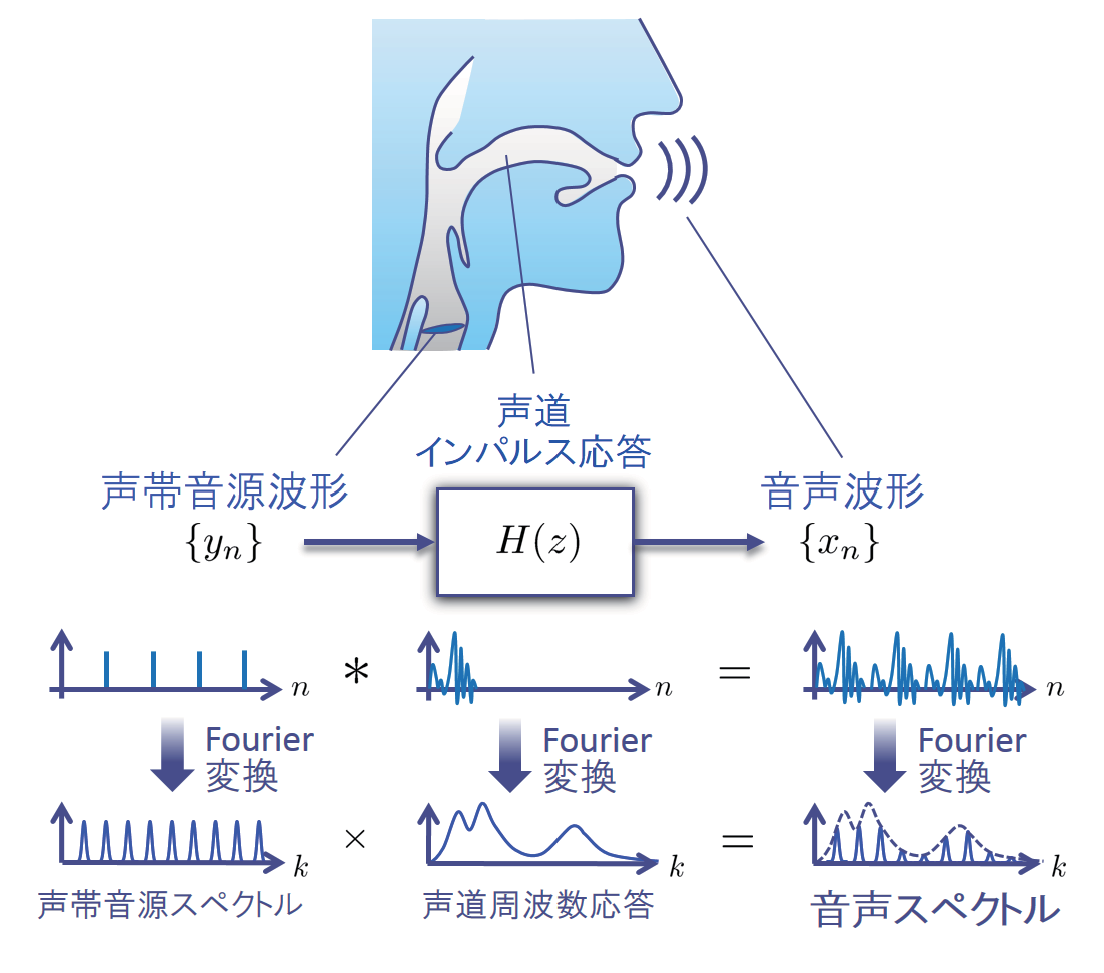
\includegraphics[width=.98\linewidth,keepaspectratio=true]{sections/speech/sourcefiltermodel3.eps}
\vspace{0ex}
 \caption{ソースフィルタ理論による音声生成過程モデル}
\label{fig:sourcefiltermodel}
\vspace{0ex}
\end{figure}

音声信号は,声帯によって発せられ声道による共振を受けた音波が,口唇から放射されたものです.
声道を線形フィルタと見なせば音声信号は声帯音源信号を入力した線形系の応答と見なせます(\reffig{sourcefiltermodel}).
このような音声信号の生成過程のモデル化は{\bf ソースフィルタ理論}と呼ばれています\cite{Chiba1941,Fant1960}.
予測誤差$\{y_n\}$を声帯音源信号,
予測係数$\Vec{a} = (a_1,\cdots,a_P)^{\mathsf T}$を
声道のフィルタ特性(声道スペクトル)を特徴付けるパラメータと見なせば,線形予測分析は
ソースフィルタ理論の解釈の下で
周波数領域において音声の声道スペクトル推定を行っていることに相当します.
以下ではこのことを示します.


音声信号$\{x_n\}$と予測誤差系列$\{y_n\}$の関係は
\begin{align}
y_n = x_n - \sum_{p=1}^{P} a_p x_{n-p}
\end{align}
で与えられます.$X(z)$と$Y(z)$をそれぞれ$\{x_n\}$と$\{y_n\}$の
$z$変換(?章参照)とすると,
\begin{align}
Y(z) &= A(z)X(z)\\
A(z) &= 1 - a_1 z^{-1} - a_2 z^{-2} \cdots - a_P z^{-P}
\end{align}
となるため,音声信号を入力として予測誤差系列を出力とする系は$A(z)$
を伝達関数とする線形時不変系で表されます.
逆に,予測誤差系列$\{y_n\}$を入力として音声信号$\{x_n\}$を出力とする
系の伝達関数は$A(z)$の逆数
\begin{align}
H(z) = \frac{1}{A(z)}
\end{align}
となります.この伝達関数は零をもたず極のみをもちますが,
?章で述べたとおり
このように極のみからなるシステムを全極システムといいます.
すなわち,もし音声信号の生成過程が線形時不変系で表せて,
予測誤差系列$\{y_n\}$を声帯音源信号と見なすことができれば,
声道の共振特性を全極型の伝達関数で表現していることになります.
$k=1,\ldots,N$を周波数インデックスとすると,
$z$変換において$z = e^{2\pi\j(k-1)/N}$としたものは離散Fourier変換
と一致します.従って,
$H(e^{2\pi\j(k-1)/N})$は全極システムの周波数応答となります.
また,$|H(e^{2\pi\j(k-1)/N})|^2$を全極スペクトルと呼びます.
実は声道フィルタとして全極システムを仮定することは
声道を無損失系の等長音響管でモデル化していることに相当します.
このことは\refsubsec{acoustic_cube_model}で詳しく述べることにして,
ここでは線形予測分析が周波数領域で何を行っていることに相当するのか
を明らかにします.

\refsubsec{TD_LPC}では
線形予測分析は時間領域では\refeq{s_pdf}を尤度関数とした予測係数$\Vec{a}$
の最尤推定問題として定式化されることを示しました.ここでは,$\Vec{x}$
の離散Fourier変換の尤度関数を導きます.
$\Vec{F}$を各行に異なる周波数の
複素正弦波が格納された離散Fourier変換行列
\begin{align}
\Vec{F} 
%&= (e^{e^{2\pi\j k n /N}})_{k,n}\\ 
&=
\frac{1}{\sqrt{N}}
\begin{bmatrix}
1&1&1&\cdots&1\\
1&e^{2\pi\j1/N}&e^{2\pi\j2/N}&\cdots&e^{2\pi\j(N-1)/N}\\
\vdots&\vdots&\vdots& &\vdots\\
1&\!\!e^{2\pi\j(N-1)/N}\!\!&\!\!e^{2\pi\j(N-1)2/N}\!\!&\!\!\cdots\!\!&\!\!e^{2\pi\j(N-1)(N-1)/N}
\end{bmatrix}
\end{align}
とすると,
$\Vec{x}$の離散Fourier変換は${\Vec{\chi}} = \Vec{Fx}$
で与えられ,$\Vec{\chi}=(\chi_1,\ldots,\chi_N)^{\mathsf T}$
の第$k$要素は周波数$k$の成分を表します.
$\Vec{F}$はユニタリ行列で
$|\det(\Vec{F})|=1$なので,確率密度関数の変数変換により,$\Vec{\chi}$は
平均が$\Vec{0}$,
分散共分散行列が$\sigma^2 \Vec{F}\Vec{\Psi}^{-1}\Vec{\Psi}^{- \mathsf T}\Vec{F}^{\mathsf H}$
の複素正規分布に従います.
\begin{align}
\Vec{\chi} \sim \mathcal{N}_{\mathbb{C}}(\Vec{\chi};\Vec{0},\sigma^2 
\Vec{F}\Vec{\Psi}^{-1}\Vec{\Psi}^{- \mathsf T}\Vec{F}^{\mathsf H})
\label{eq:c_pdf}
\end{align}
ただし,$\mathcal{N}_{\mathbb{C}}(\Vec{x};\Vec{\mu},\Vec{\Sigma}) = \frac{1}{\pi^N |\det(\Vec{\Sigma})|}e^{-(\Vec{x}-\Vec{\mu})^{\mathsf H}\Vec{\Sigma}^{-1}(\Vec{x}-\Vec{\mu})}$です.
ここで,分析窓の両端点において信号が巡回していると仮定し,
\refeq{Psi}の代わりに$\Vec{\Psi}$を
\begin{align}
\Vec{\Psi} = 
\begin{bmatrix}
\hspace{-0ex}1& & &\hspace{-1.7ex}-a_P&\hspace{-1.7ex}\cdots&\hspace{-1.7ex}-a_1\vspace{-1.7ex}\\
\hspace{-0ex}-a_1&\hspace{-1.7ex}\ddots& & &\hspace{-1.7ex}\ddots&\hspace{-1.7ex}\vdots\vspace{-1.7ex}\\
\hspace{-0ex}\vdots&\hspace{-1.7ex}\ddots&\hspace{-1.7ex}\ddots& & &\hspace{-1.7ex}-a_P\vspace{-1.7ex}\\
\hspace{-0ex}-a_P& &\hspace{-1.7ex}\ddots &\hspace{-1.7ex}\ddots& &\vspace{-1.7ex}\\
 &\hspace{-1.7ex}\ddots& &\hspace{-1.7ex}\ddots&\hspace{-1.7ex}\ddots&\vspace{-1.7ex}\\
\hspace{-0ex}0 & &\hspace{-1.7ex}-a_P&\hspace{-1.7ex}\cdots&\hspace{-1.7ex}-a_1&\hspace{-1.7ex}1
\end{bmatrix}
\label{eq:Psi2}
\end{align}
のような巡回行列とします.巡回行列同士の積は巡回行列になり,また,
巡回行列は離散Fourier変換行列により対角化されるため,
\begin{align}
\sigma^2
\Vec{F}\Vec{\Psi}^{-1}\Vec{\Psi}^{- \mathsf T}\Vec{F}^{\mathsf H}
&=\sigma^2(\Vec{F}\Vec{\Psi}^{\mathsf T}\Vec{\Psi} \Vec{F}^{\mathsf H})^{-1}
\nonumber\\
&= {\rm diag}(\lambda_1,\ldots,\lambda_T)
\label{eq:diagonalize}
\end{align}
となります.ただし,$\lambda_k$は$\sigma^2\Vec{\Psi}^{-1}\Vec{\Psi}^{- \mathsf T}$
の固有値
\begin{align}
\lambda_k &= \frac{\sigma^2}{|A(e^{2\pi\j(k-1)/N})|^2}\label{eq:allpole}\\
A(z) &= 1- a_1z^{-1} - \cdots -a_P z^{-P}
\end{align}
で与えられ,周波数$k$における全極スペクトルを表します.
\refeq{c_pdf}および\refeq{diagonalize}より,所与の$\Vec{\chi}$の下での$\Vec{a}$の対数尤度は
\begin{align}
\log p(\Vec{\chi}|\Vec{a}) = 
- \sum_k 
\left(\log \pi \lambda_k
+
\frac{|\chi_k|^2}{\lambda_k} 
\right)
\label{eq:X_loglikelihood}
\end{align}
となり,もし$\lambda_k$に何も制約がなく$k$ごとに自由度をもつならば
\begin{align}
\frac{\partial \log p(\Vec{\chi}|\Vec{a})}{\partial \lambda_k}=
-
\frac{1}{\lambda_k} 
+
\frac{|\chi_k|^2}{\lambda_k^2}
=0
~~
\Rightarrow
\lambda_k=|\chi_k|^2
\end{align}
より,
$\lambda_k=|\chi_k|^2$のときに最大になります.よって,\refeq{X_loglikelihood}に
$\lambda_k=|\chi_k|^2$を代入したものから\refeq{X_loglikelihood}を引いたもの
\begin{align}
D_{\rm IS}(\lambda_k\||\chi_k|^2) &=
- 
\sum_k 
\left(\log \pi |\chi_k|^2
+
1
\right)
+
\sum_k 
\left(\log \pi \lambda_k
+
\frac{|\chi_k|^2}{\lambda_k} 
\right)
\nonumber\\
&=
\sum_k 
\left( 
\frac{|\chi_k|^2}{\lambda_k} - \log \frac{|\chi_k|^2}{\lambda_k} - 1
\right)
\nonumber\\
&\ge 0
\label{eq:ISdivergence}
%\sum_k D_{\rm IS}(\lambda_k\||x_k|^2)\\
%D_{\rm IS}(y|x) = \frac{x}{y} - \log \frac{x}{y} - 1
\end{align}
は信号のパワースペクトル$|\chi_k|^2$と全極スペクトル$\lambda_k$の離れ具合を表す非負の尺度となります.
これを{\bf 板倉齋藤距離}と呼びます\cite{Itakura1972}.\reffig{ISdivergence}を見ても分かるように,
板倉齋藤距離は\footnote{よって,板倉齋藤距離は距離の公理を満たさないので
厳密には距離ではありませんが、伝統的にこのように呼ばれています.
板倉齋藤歪みや板倉齋藤ダイバージェンスという呼称も見られます.}{非対称}で,
$\lambda_k$が$|\chi_k|^2$を下回る場合により過大なペナルティを課す
誤差関数です.
このため\refeq{ISdivergence}は,
$\lambda_k$が
$|\chi_k|^2$をできるだけ下回らず
$|\chi_k|^2$のピークの近くを通るような関数となっているときほど小さい値になります.
通常,線形予測分析により音声分析を行う際,次数$P$は10から20程度に設定することが多いですが,
この場合,線形予測分析では音声のスペクトルの包絡線(スペクトル包絡)を推定していると見なすことができます.
実際,\reffig{AllPoleFitting}を見ると,たしかに全極スペクトルが音声スペクトルのピークの近くを通るように推定されていることが分かります.

さて,
\refeq{X_loglikelihood}を最大化する$\Vec{a}$が
時間領域で求めた最尤解と同じになることを確認しておきましょう.
証明は例えば\cite{Sugiura2015}に譲りますが,$N \gg P$においては$\Vec{\Psi}$が
\refeq{Psi2}のような巡回行列で与えられる場合でも
$\det(\Vec{\Psi})\simeq 1$となることが示せるので,
\refeq{diagonalize}の左辺の行列式は
$\det(\sigma^2 \Vec{F} \Vec{\Psi}^{-1}\Vec{\Psi}^{-\mathsf T} \Vec{F}^{\mathsf H}) = 
\sigma^{2N} \det(\Vec{F})^2 \det(\Vec{\Psi})^{-2}\simeq\sigma^{2N}$と近似できます.
また,右辺の行列式は$\prod_k \lambda_k$となるので
$\sum_k \log \lambda_k = N \log \sigma^2$が言えます.
従って,\refeq{X_loglikelihood}は
\begin{align}
\log p(\Vec{\chi}|\Vec{a}) = 
- N \log (\pi\sigma^2)
- \sum_k 
\frac{|\chi_k|^2 }{\sigma^2}
\bigg|1 - \sum_p a_p e^{ - 2\pi\j p(k-1)/N} \bigg|^2 
\end{align}
と書けます.対数尤度$\log p(\Vec{\chi}|\Vec{a})$の$a_q$に関する偏微分
\begin{align}
\frac{\partial \log p(\Vec{\chi}|\Vec{a})}{\partial a_q}&=
\sum_k \frac{|\chi_k|^2 }{\sigma^2}
2{\rm Re}\left[
e^{ 2\pi\j q(k-1)/N} - \sum_p a_p e^{2\pi\j (q-p)(k-1)/N}
\right] 
\nonumber
\end{align}
を0と置いた式
\begin{align}
\sum_p a_p 
{\rm Re}\left[
\sum_k |\chi_k|^2
e^{2\pi\j (q-p)(k-1)/N}
\right]
=
{\rm Re}\left[
\sum_k |\chi_k|^2 e^{ 2\pi\j q(k-1)/N}
\right]
\nonumber
\end{align}
を$q = 1,\ldots,P$について連立させることで,
最尤の$\Vec{a}$が満たすべき方程式
\begin{align}
\begin{bmatrix}
v_{0} & v_{-1} & \cdots & v_{1-P}\\
v_{1} & v_{0} & \cdots & v_{2-P}\\
\vdots & \vdots & \ddots & \vdots\\
v_{P-1} & v_{P-2} & \cdots & v_{0}
\end{bmatrix}
\begin{bmatrix}
a_1\\
a_2\\
\vdots\\
a_P
\end{bmatrix}
=
\begin{bmatrix}
v_{1}\\
v_{2}\\
\vdots\\
v_{P}
\end{bmatrix}
\label{eq:lpc_YuleWalker3}
\\
v_{q}=
{\rm Re}\left[
\sum_k |\chi_k|^2 e^{ 2\pi\j q(k-1)/N}
\right]
\label{eq:v_q}
\end{align}
が得られます.
ここで,
\refeq{v_q}は音声信号$\{x_n\}$のパワースペクトル$\{|\chi_k|^2\}$の
逆Fourier変換となっているため,
$\{v_q\}$は\refeq{lpc_YuleWalker2}における$\{v_q\}$と同様,$\{x_n\}$の
自己相関関数を表す変数となっています.
また,
$\{|\chi_k|^2\}$は実関数なので,$\{v_q\}$は偶関数($v_q = v_{-q}$)
となります.
よって,\refeq{lpc_YuleWalker3}は
\refeq{lpc_YuleWalker2}と同じ形のYule-Walker方程式に帰着します.






\begin{figure}[t!]
\centering
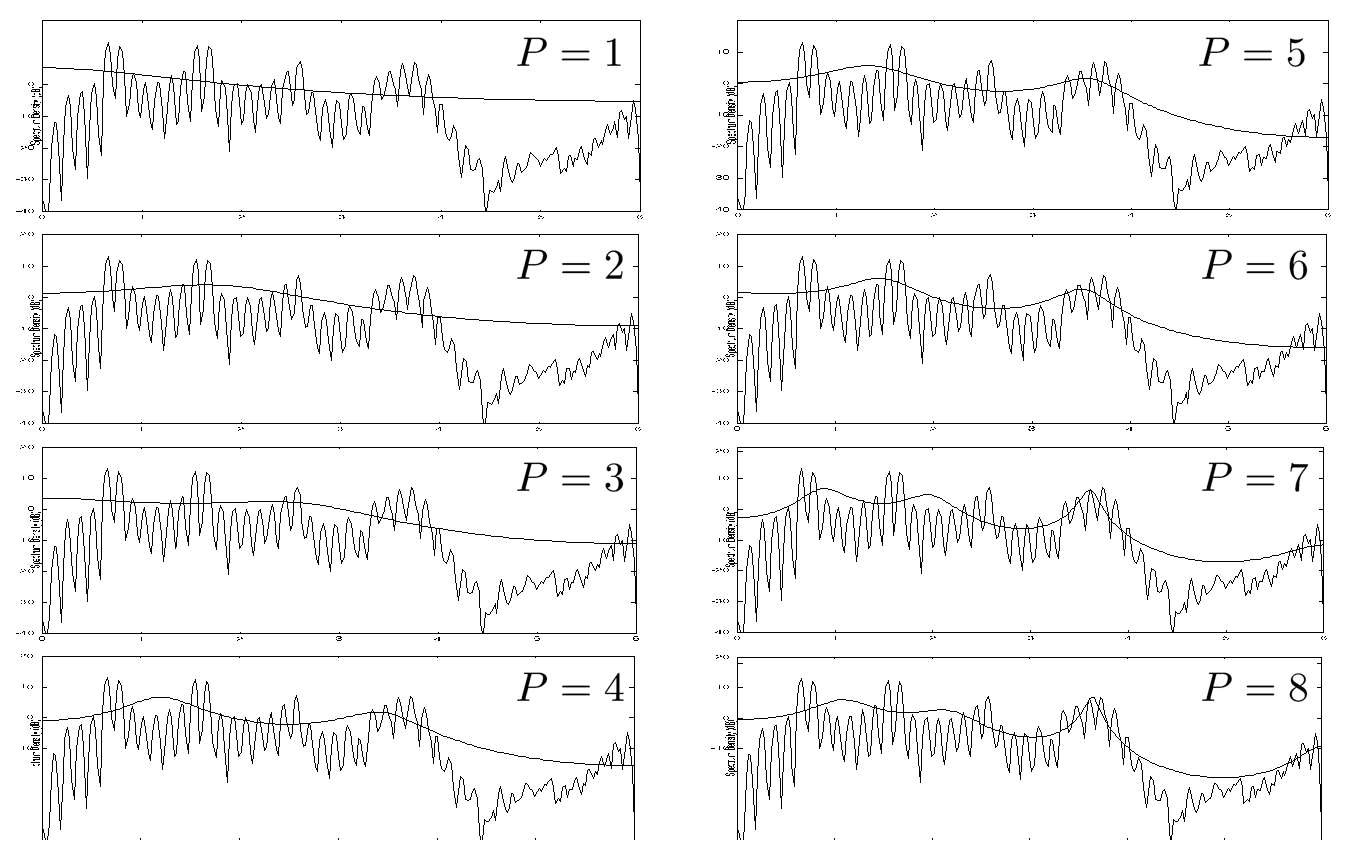
\includegraphics[width=.98\linewidth,keepaspectratio=true]{sections/speech/AllPoleFitting1.eps}
%\caption{音声スペクトルと次数$P$の線形予測分析により推定された全極スペクトル($P=1,\ldots,8$)}
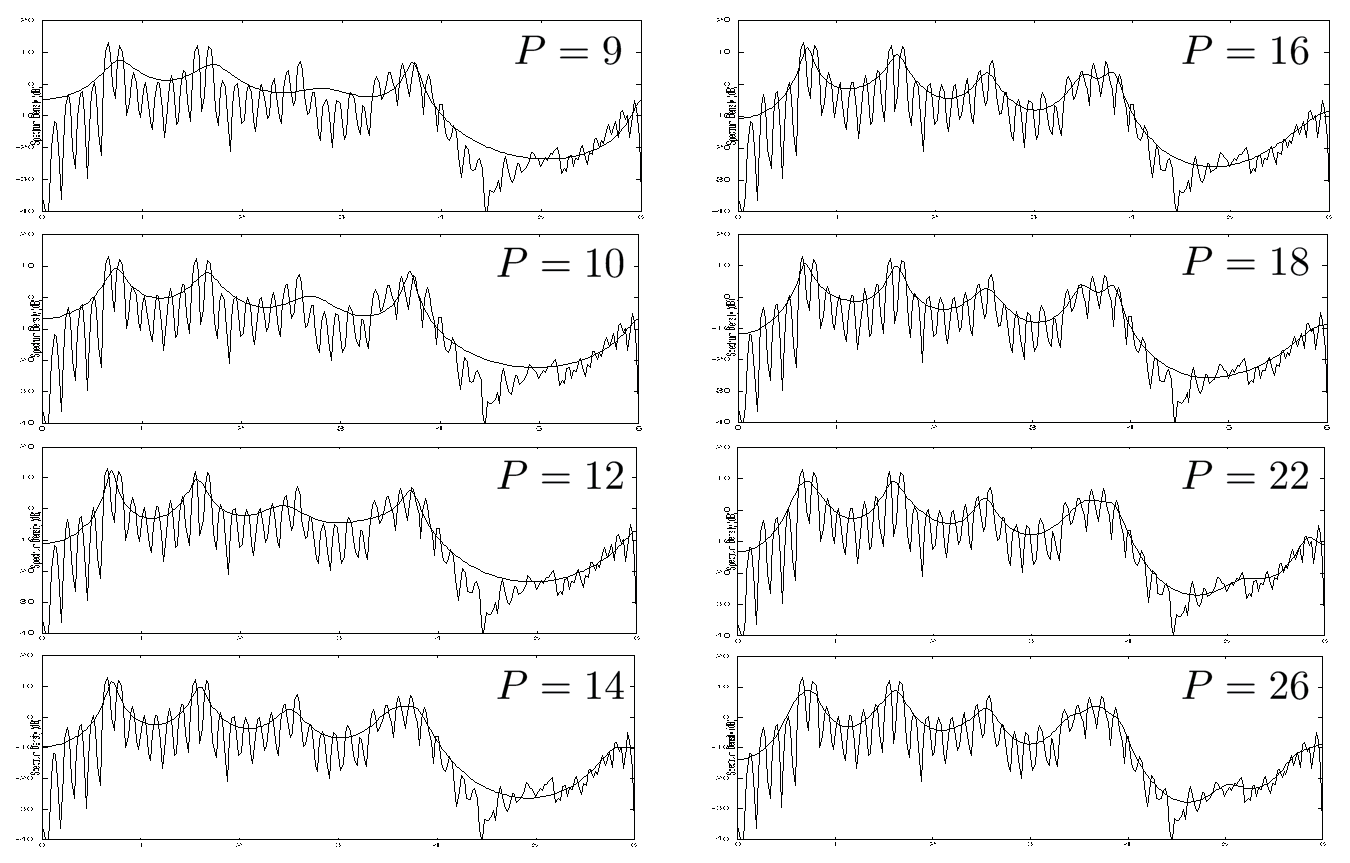
\includegraphics[width=.98\linewidth,keepaspectratio=true]{sections/speech/AllPoleFitting2.eps}
\vspace{0ex}
 \caption{音声スペクトルと次数$P$の線形予測分析により推定された全極スペクトル($P=1,\ldots,8,9,10,12,14,16,18,22,26$)}
\label{fig:AllPoleFitting}
\vspace{0ex}
\end{figure}

\subsection{無損失系等長音響管による声道モデルとしての解釈}
\label{subsec:acoustic_cube_model}

本節では全極システムを仮定することが無損失系等長音響管により声道をモデル化していることに相当することを示します.
%線形予測分析の手法にのみ関心のある読者は本節は読み飛ばしていただいて差し支えありません.
そこでまず,一定の断面積の管の中を進行する音波の波動方程式を導き,
これをもとに,断面積が不連続に変化する管内を音波がどう伝播していくかを考えます.

音波は空気などの媒質の中を伝播する粗密波で,
%粗密波の伝播速度を音速,
平均圧力を基準として音波によって引き起こされる圧力の変化分を音圧といいます.
空間中のある断面に圧力変動が伝わると,その断面上で,媒質を構成する微小粒子が平衡位置から変位させられます.
このときの粒子の速度を粒子速度といいます.
音波は音圧と粒子速度の二つの量によって特徴付けられ,
これらの量を支配する方程式を波動方程式と呼びます.
ここでは,断面積が$S$で$d$軸方向に伸びている管を考え,
この管と$d$と$d+\Delta d$の二つの面で囲まれた微小部分(\reffig{waveq})における
音圧と粒子速度の関係を導くため,
媒質の運動量の保存を表す運動方程式と
質量の保存を表す連続の方程式を導入します.


まず運動方程式を導きます.
時刻$t$における$d$での音圧を$P(t,d)$とすれば$d+\Delta d$での音圧は$P(t,d) + \frac{\partial P(t,d)}{\partial d} \Delta d$となります.
ゆえに,この微小部分には左右逆向きの力$P(t,d)S$と$(P(t,d) + \frac{\partial P(t,d)}{\partial d} \Delta d)S$
が加わるので,その差の力$- \frac{\partial P(t,d)}{\partial d} \Delta d S$により
微小部分の粒子が動かされます.
管内の媒質の密度を$\rho$とすると微小部分の質量は$\rho\Delta d S$になり,さらに
粒子の変位を$\zeta(t,d)$とすると粒子の加速度は$\frac{\partial^2 \zeta(t,d)}{\partial t^2}$になるので,
\begin{align}
-\frac{\partial P(t,d)}{\partial d}\Delta d S = \rho \Delta d S \frac{\partial^2 \zeta(t,d)}{\partial t^2}
\end{align}
という運動方程式を得ます.
この式に粒子速度$v(t,d) = \frac{\partial \zeta(t,d)}{\partial t}$を代入した
\begin{align}
-\frac{\partial P(t,d)}{\partial d} &= \rho \frac{\partial v(t,d)}{\partial t}
\label{eq:moteq}
\end{align}
が音圧と粒子速度の関係を表す一つ目の式となります.

\begin{figure}[t!]
\centering
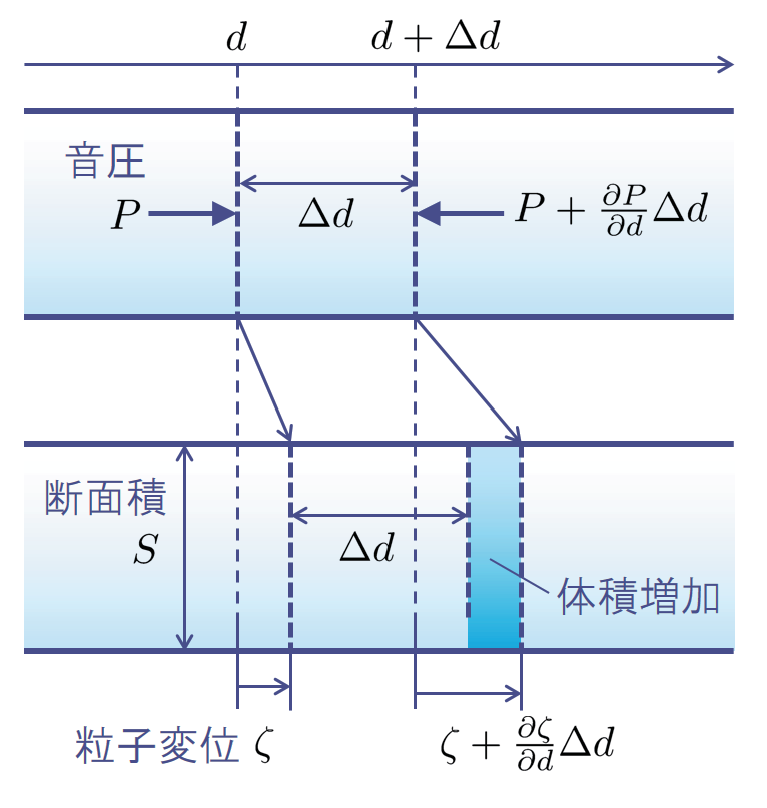
\includegraphics[width=.55\linewidth,keepaspectratio=true]{sections/speech/acoustictube.eps}
\vspace{0ex}
 \caption{***}
\label{fig:waveq}
\vspace{0ex}
\end{figure}


次に連続の方程式を導きます.
上記運動方程式に従って
$d$の位置にあった粒子が$\zeta(t,d)$だけ変位したとすると,$d+\Delta d$にあった粒子
の変位は$\zeta(t,d) + \frac{\partial \zeta(t,d)}{\partial d}\Delta d$となります.
よって,微小部分の体積$\Delta d S$は変位の差と断面積の積
$\frac{\partial \zeta(t,d)}{\partial d}\Delta d S$だけ膨張します.
媒質の体積減少の割合$(\frac{\partial \zeta(t,d)}{\partial d}\Delta d S) / (\Delta d S)$
は加えられた圧力$P(t,d)$に比例するので,比例定数を$K$とすると
\begin{align}
P(t,d) = -K \frac{\partial \zeta(t,d)}{\partial d}
\end{align}
という関係式が得られます.$K$は体積弾性率と呼ばれ,媒質によって決まる値です.
この式の両辺を時間$t$で微分し,粒子速度$v(t,d) = \frac{\partial \zeta(t,d)}{\partial t}$を代入すると
\begin{align}
-\frac{\partial P(t,d)}{\partial t} = K \frac{\partial v(t,d)}{\partial d}
\label{eq:conteq}
\end{align}
という式を得ます.これが連続の方程式で,音圧と粒子速度の関係を表す二つ目の式となります.
%体積速度$u(t,d) = S v(t,s)$

これらの二つの関係式を同時に記述したものが波動方程式です.そこで,両式を統合化することを考えます.
\refeq{moteq}の両辺を$d$で微分した式と\refeq{conteq}の両辺を$t$で微分した式を用いれば,
$v$を消去し$P$だけの式に書き換えることができます.逆に,
\refeq{moteq}の両辺を$t$で微分した式と\refeq{conteq}の両辺を$d$で微分した式を用いることで
$v$だけの式に書き換えることができます.この操作により$P$と$v$に関する波動方程式
\begin{align}
\frac{\partial^2 P(t,d)}{\partial d^2} &= \frac{1}{c^2} \frac{\partial^2 P(t,d)}{\partial t^2}
\\
\frac{\partial^2 v(t,d)}{\partial d^2} &= \frac{1}{c^2} \frac{\partial^2 v(t,d)}{\partial t^2}
\\
c &=\sqrt{\textstyle\frac{K}{\rho}}
\end{align}
を得ます.
%後述するように$c$は音速に対応します.従って,音速$c$は
%媒質の体積弾性率$K$と密度$\rho$によって決まる定数であることが分かります.
これらの式は$P$と$v$の振る舞いを別々に表現したもので,
両者の関係を記述した形にはなっていません.
そこで,$P$と$v$の関係を記述しやすくする目的で
\begin{align}
v(t,d) &=
- \frac{\partial \phi(t,d)}{\partial d}
\label{eq:def_velpot}
\end{align}
を満たす速度ポテンシャルと呼ぶ関数$\phi(t,d)$を導入します.
\refeq{def_velpot}を運動方程式(\refeq{moteq})に代入し,
$d$に関して積分すると
\begin{align}
P(t,d) &=
\rho \frac{\partial \phi(t,d)}{\partial t} + C
\end{align}
を得ます.
ここで,$C$は積分定数ですが,
音波が伝播していない$\phi=0$のとき音圧が$P=0$となるように$C=0$と設定することで
\begin{align}
P(t,d) &=
\rho \frac{\partial \phi(t,d)}{\partial t}
\label{eq:def_velpot2}
\end{align}
を得ます.
\refeqs{def_velpot}{def_velpot2}より,
速度ポテンシャル$\phi(t,d)$は
$P$と$v$を結びつける関数となっていることが分かります.
あとは\refeqs{def_velpot}{def_velpot2}を連続の方程式(\refeq{conteq})に代入することで,
$P$と$v$に関する波動方程式を速度ポテンシャル$\phi(t,d)$を介して
\begin{align}
\frac{\partial^2 \phi(t,d)}{\partial d^2} = 
\frac{1}{c^2}\frac{\partial^2 \phi(t,d)}{\partial t^2} 
\label{eq:waveq}
\end{align}
のように一つの方程式で記述することができます.
***の場合の\refeq{waveq}の解は
\begin{align}
\phi(t,d) = A e^{j\omega(t-d/c)} + B e^{j\omega(t+d/c)}
\end{align}

以上より,一定の断面積の管内を一方向に伝播する音波の波動方程式は
断面積$S$に依存しないことが分かりましたが,以下で
断面積が不連続変化する音響管を伝播する音波の振る舞いを考えるため,
粒子速度$v(t,d)$の代わりに断面積$S$に依存する
体積速度$u(t,d) = S v(t,d)$という量を扱います.

\begin{figure}[t!]
\centering
%\includegraphics[width=.55\linewidth,keepaspectratio=true]{sections/speech/nonuniformacoustictube.eps}
\vspace{0ex}
 \caption{***}
\label{fig:AcousticTubeModel}
\vspace{0ex}
\end{figure}

今,\reffig{AcousticTubeModel}のように
長さが等しく断面積が異なる$M$個の管を連結した非一様音響管を考え,この管内を
長さ方向にのみ伝播する音波を考えます.
$m$番目の区間の管の断面積を$S_m$とすると,この管内を伝播する音波の速度ポテンシャル$\phi_m(t,d)$は
\begin{align}
\frac{\partial^2 \phi_m(t,d)}{\partial d^2} = 
\frac{1}{c^2}\frac{\partial^2 \phi_m(t,d)}{\partial t^2} 
\label{eq:waveq2}
\end{align}
を満たし,一般解は
\begin{align}
\phi_m(t,d) = A e^{j\omega(t-d/c)} + B e^{j\omega(t+d/c)}
\end{align}
で与えられます.
体積速度$u_m(t,d)$と速度ポテンシャル$\phi_m(t,d)$の関係は
\begin{align}
u_m(t,d) &=
- S_m \frac{\partial \phi_m(t,d)}{\partial d}
\label{eq:def_volvel}
\end{align}
で与えられ,
音圧$P_m(t,d)$と速度ポテンシャル$\phi_m(t,d)$の関係は
\refeq{def_velpot2}で与えられるので,
\begin{align}
u_m(t,d) &= u^+_m(t,d) - u^-_m(t,d)
\\
P_m(t,d)&=\frac{\rho c}{S_m}
(u^+_m(t,d) + u^-_m(t,d))
\end{align}
となります.
ただし,$u^+_m(t,d)$, $u^-_m(t,d)$は
\begin{align}
u^+_m(t,d)&=
\frac{j\omega S_m A}{c}e^{j\omega(t-d/c)}
\\
u^-_m(t,d)&=
\frac{j\omega S_m B}{c}e^{j\omega(t+d/c)}
\end{align}
で与えられます.



\section{韻律分析合成}

\subsection{背景と目的}

普段我々私たちは会話をするとき言葉を使って相手にメッセージを伝えますが,言葉とともに声の高低を効果的に使いながら声に表情をつけ,声の調子や意図や,その人っぽさなどのさまざまな情報を相手に伝えています.

声の高低の時間変化を表す基本周波数パターンは大きく分けて
フレーズ成分とアクセント成分と呼ぶ二つの成分からなります.
フレーズ成分とは文や句の全体に及ぶ範囲で緩やかに変化する基本周波数パターンのことで,話者の調子や意図,文の区切りや係り受けを表現するのに重要な役割を担います.
一方,アクセント成分とは各単語の中で急峻に変化する基本周波数パターンのことで,単語の意味や方言の違いに関係します.例えば「はし」という単語は「は」が高い場合と低い場合とでは意味が違いますし,「おいおい」という単語も先頭の「お」が高い場合と低い場合とで意味が違います.特に日本語の場合,単語アクセントと単語の意味の関係は方言によって異なるので,単語内の基本周波数パターンを変えて話せば異なった方言になります.また,フレーズ成分とアクセント成分の大きさは,文や句や単語の強弱を表すいわゆるメリハリに相当します.これらが大きい場合と小さい場合とでは話し方の印象は大きく変わり,メリハリをつけることで発話の中で注目すべき文や単語を相手に示すことができるようになります.以上のように,基本周波数パターンは様々さまざまな情報を持っており,言葉に勝るとも劣らないくらい音声コミュニケーションにおいて大きな役割を果たしています.
基本周波数パターン分析とは,***。

%甲状軟骨による基本周波数制御
基本周波数パターンは声帯を伸縮させる甲状軟骨という部位により制御されています.
藤崎らによってこの制御メカニズムを模擬した物理モデルが提案されており(\reffig{Fujisakimodel}),藤崎モデルと呼ばれています.
甲状軟骨の運動がどのような基本周波数パターンをもたらすかを簡潔に説明した方程式で,日本語を含む多言語の音声の基本周波数パターンを極めて良く表現できることが知られています.このモデルでは,甲状軟骨の二つの独立な運動(並進と回転)に伴う声帯の長さの変化の合計と対数基本周波数の変化が比例関係にあり,それぞれの運動がイントネーションとアクセントに関与しているという仮定がベースとなっています.このモデルに基づき,音声から甲状軟骨がどう動いたかを推定することができれば,その声にそっくりの基本周波数パターンを再現することができ,さらにその数値を変えてやれば甲状軟骨が異なる動きをした場合の基本周波数パターンの音声を再合成することができるようになります.ところが,この逆問題は一筋縄ではいかず長らく未解決問題とされていました.例えば7+3を解くのは簡単でもX+Y=10となるXとYを一意に決められないのと同じで,フレーズ成分とアクセント成分から基本周波数パターンを得る方程式は与えられていたとしても基本周波数パターンのみからフレーズ成分とアクセント成分を一意に決めることはできないからです.しかしまったく全く手がかりがないわけではありません.自然音声におけるフレーズやアクセントのタイミングや強度には統計的な偏りがあります.藤崎モデルの確率モデル化により
統計的アプローチにより基本周波数パターンから藤崎モデルのパラメータを推定する
(フレーズ成分とアクセント成分に分解する)手法が
亀岡らによって提案されています.
\refsubsec{OriginalFujisakiModel}以降で,藤崎モデルについて概説した上で
亀岡らの手法を紹介します.

\subsection{骨格筋の弾性特性}

藤崎モデルでは,
\begin{enumerate}
\item 声帯の伸びの合計と対数基本周波数の変化が比例関係にある
\item 対数基本周波数がフレーズ成分とアクセント成分とベースライン成分の三成分の和で表される
\end{enumerate}
という二つの重要な仮定がベースとなっていました.
これらの仮定の妥当性に対する藤崎による説明は以下のとおりです.

$l$を筋肉の長さとすると,
声帯筋を含む骨格筋において,長さ方向に加わる張力$T$と
剛性${\mbox{d}T}/{\mbox{d}l}$(筋肉を単位長さ変化させるのに必要な力)の間には
\begin{align}
\frac{\mbox{d}T}{\mbox{d}l} = a + b T
\end{align}
のような線形の関係が成り立つことが多くの実測結果により示されています
\cite{Buchthal1944,Sandow1958}.
ただし,$a$は$T=0$における筋肉の剛性です.
声帯筋の静止張力を$T_0$とし,そのときの声帯筋の長さを$l_0$とすると,
この微分方程式より張力$T$と声帯筋の長さ$l$の関係を表す式
\begin{align}
T = \left(T_0 + \frac{a}{b}\right) e^{b(l-l_0)} - \frac{a}{b}
\label{eq:stress-strain}
\end{align}
が導かれます.ここで,$T_0 \gg a/b$のとき,\refeq{stress-strain}は
\begin{align}
T = T_0 e^{b\delta}
\label{eq:stress-strain2}
\end{align}
と近似できます.
ただし,$\delta = l-l_0$は張力が$T_0$から$T$へ変化した際の声帯筋の長さの変化を表します.
一方,一定の張力$T$で張られた密度$\rho$の
弾性膜の固有振動周波数$f_0$は,膜の大きさによって決まる定数$c_0$を用いて
\begin{align}
f_0 = c_0 \sqrt{T/\rho}
\label{eq:F0_tension}
\end{align}
と表されます.
従って,
\refeq{stress-strain2}と\refeq{F0_tension}より,
声帯の伸びが$\delta$のときの基本周波数の対数$y = \log f_0$は
\begin{align}
%f_0 = c_0 \sqrt{T_0 e^{bx} / \rho}%\\
y = \log c_0 \sqrt{T_0/\rho} + \frac{b}{2}\delta
\end{align}
となり,$\delta$と$y$が線形の関係にあることが示されます.
声帯の伸び$\delta$が時間変化する場合,$t$を時刻とすると
基本周波数パターン$y(t)$は
\begin{align}
y(t) &= \log c_0 \sqrt{T_0/\rho} + \frac{b}{2}\delta(t)
\end{align}
のように固定項と時間変化成分
の和として表されます。

声帯の長さは甲状軟骨の平行移動運動と回転運動によって変化します.
平行移動運動によって生じる変化分を$\delta_{\rm p}(t)$,
回転運動によって生じる変化分を$\delta_{\rm a}(t)$とすると,
これらの二つの運動が微小で互いに独立と見なせる範囲では
声帯の長さの変化は$\delta_{\rm p}(t)$と$\delta_{\rm a}(t)$の和
となります.
なお,甲状軟骨の平行移動の時定数は,回転の時定数よりもはるかに大きいため,
多くの言語に共通する特徴として$\delta_{\rm p}(t)$が句単位の比較的緩やかな音調の表現に,
$\delta_{\rm a}(t)$が語または音節単位の比較的急激で局所的な音調の表現に用いられています.


\subsection{基本周波数パターン生成過程モデル\cite{Fujisaki1988}}
\label{subsec:OriginalFujisakiModel}
%\vspace{-1ex}

%ここでは藤崎モデルを概説する。
%藤崎モデルは,音声における$F_0$の対数値の時間軌跡($F_0$パターン)
%を喉頭の生理的,物理的特性に基づいてモデル化したものである。
藤崎モデルでは,
%次のような考え方に基づく。
%甲状軟骨の運動には平行移動と回転の二つの自由度があり,
%それぞれの運動に伴って声帯の長さが変化する。
%声帯の長さの伸びは,これら二つの変化
%の和で表される。
甲状軟骨の二つの独立な運動(平行移動と回転)
に伴う声帯の長さの変化の合計が
$F_0$の時間的変化をもたらす
と解釈され,声帯の伸び
と対数$F_0$の変化が比例関係にあるという仮定
に基づき$F_0$パターンがモデル化されます.


甲状軟骨の平行移動運動に関係する
$F_0$パターンをフレーズ成分,
回転運動に関係する$F_0$パターンを
アクセント成分と呼び,
それぞれ$y_{\rm p}(t)$, $y_{\rm a}(t)$とします。
ただし,$t$は時刻です。
$y_{\rm p}(t)$の生成過程(フレーズ制御機構)
はフレーズ指令と呼ぶ
パルス波を入力とした臨界制動の二次線形系,
$y_{\rm a}(t)$の生成過程(アクセント制御機構)
はアクセント指令と呼ぶ
矩形波を入力とした臨界制動の二次線形系に
より表現されます.
以上の二つの成分と,
声帯の物理的性質によって決まる
ベースライン成分$y_b$の和$y_{\rm p}(t)+y_{\rm a}(t)+y_b$
で$F_0$パターン$y(t)$を表したものが藤崎モデルです.
フレーズ成分は短区間の上昇のあとに緩やかな下降をなす成分で,
アクセント成分は急激な上昇下降をなす成分であるため,
多くの言語に共通して
前者が句単位の比較的緩やかな音調を,
後者が語または音節単位の比較的急激で局所的な
音調を表現する役割を担っていると考えられています.
フレーズ制御機構およびアクセント制御機構は
\begin{align}
G_{\rm p}(t)&=
\begin{cases}
\alpha^2 t e^{-\alpha t}&(t\ge 0)\\
0&(t<0)
\end{cases}
%\nonumber
%\end{align}
\\
%\begin{align}
G_{\rm a}(t)&=
\begin{cases}
\beta^2 t e^{-\beta t}&(t\ge 0)\\
0&(t<0)
\end{cases}
\end{align}
で与えられる
インパルス応答$G_{\rm p}(t)$, $G_{\rm a}(t)$によって
特徴づけられます.
$\alpha$と$\beta$はそれぞれの制御機構
の固有角周波数であるが,これらは話者ごとにほぼ一定値を
とること,話者の個人差も言語による差も比較的小さい
ことが確かめられており,
おおよそ$\alpha\!=\!3$rad/s, $\beta\!=\!20$rad/s
程度であることが経験的に知られています.
これらを用いて$F_0$パターン$y(t)$は具体的に
\begin{align}
\hspace{-0.0cm}
y(t) = y_{\rm b}
&+\sum_{i}A_{{\rm p},i}G_{\rm p}(t-T_{0,i})
\nonumber
\\
&+\sum_{j}A_{{\rm a},j}
\big\{S_{\rm a}(t-T_{1,j})-S_{\rm a}(t-T_{2,j})\big\}
%\nonumber
\end{align}
と表されます.
%(\reffig{fujisaki_model})
ただし,$A_{{\rm p},i}$と$T_{0,i}$は
それぞれ$i$番目のフレーズ指令の大きさと生起時刻であり,
$A_{{\rm a},j}$と$T_{1,j}$,と$T_{2,j}$は
それぞれ$j$番目のアクセント指令の振幅と始端時刻と
終端時刻を表します.
ところで,
アクセント制御機構のインパルス応答
$G_{\rm a}(t)$は$S_{\rm a}(t)$
の時間微分ゆえ
\begin{align}
G_{\rm a}(t)=
\begin{cases}
\beta^2 t e^{-\beta t}&(t\ge 0)\\
0&(t<0)
\end{cases}
\end{align}
となり,$G_{\rm p}(t)$と同形であることが分かります.
従って,アクセント成分$y_{\rm a}(t)$は複数の矩形波からなるアクセント指令関数$u_{\rm a}(t)$
と$G_{\rm a}(t)$の畳み込みによって表されます.

%\begin{figure}[t!]
%\centering
%\includegraphics[width=.98\linewidth,keepaspectratio=true]{sections/speech/fujisakimodel_ver3_ill.eps}
%\vspace{-1ex}
% \caption{Block diagram of Fujisaki model}
%\label{fig:fujisaki_model}
%\vspace{-2ex}
%\end{figure}


%\subsection{藤崎モデルの離散時間表現}
%\label{sec:DiscreteFujisaki}


本章では,藤崎モデルの離散時間表現を得るため,
連続時間システムのフレーズ制御機構およびアクセント制御機構
に対して後退差分変換により離散化を行います.
%離散化することの理由はのちに明らかにする。
まず,フレーズ制御機構の伝達関数(Laplace変換)は
$%\begin{align}
\mathcal{G}_{\rm p}(s)= 
\mathcal{L}\big[G_{\rm p}(t)\big]=
{\alpha^2}/{(s+\alpha)^2}
$%\end{align}
で与えられます.
後退差分変換は,
時間微分演算子$s$
を$z$領域における後退差分演算子
$
s\simeq
{(1-z^{-1})}/{t_{0}}
$
に置き換える変換であり($t_0$は変換先の離散時間表現における
サンプリング周期),
この変換により,
$\mathcal{G}^{-1}_{\rm p}(s)$
の逆システムの伝達関数を$z$領域で
\begin{align}
\mathcal{H}_{\rm p}^{-1}(z)&= 
a_2
%\frac{1}{\alpha^2t_{0}^2}
z^{-2}
+a_1
%-\frac{2(\alpha t_{0} +1)}{\alpha^2t_{0}^2}
z^{-1}
+a_0
%+\frac{(\alpha t_{0}+1)^2}{\alpha^2t_{0}^2}.
\end{align}
と書くことができます.
ただし,
\begin{align}
a_2 = (\psi-1)^2,~~
a_1 = -2\psi(\psi-1),~~
a_0 = \psi^2
\label{eq:a_psi}
\end{align}
および,$\psi = 1+1/(\alpha t_0)$です.
ここで,$k$を離散時刻インデックスとし,
フレーズ指令関数およびフレーズ成分の
離散時間表現をそれぞれ
$u_{\rm p}[k]$および$y_{\rm p}[k]$
とすると,$y_{\rm p}[k]$
は,単一のパラメータ$\psi$(あるいは$\alpha$)
によって特性が決まる拘束つき全極モデルからの出力
\begin{align}
&u_{\rm p}[k] = a_0 y_{\rm p}[k]+a_1y_{\rm p}[k-1]+a_2y_{\rm p}[k-2]
\end{align}
と見なすことができます.
同様に,
アクセント指令関数$u_{\rm a}[k]$
とアクセント成分$y_{\rm a}[k]$の関係も
\begin{align}
u_{\rm a}[k] &= b_0 y_{\rm a}[k]+b_1y_{\rm a}[k-1]+b_2y_{\rm a}[k-2]
\end{align}
と書くことができます.
ただし,
$b_2 = (\varphi-1)^2$, $b_1 = -2\varphi(\varphi-1)$,
$b_0 = \varphi^2$, 
$\varphi = 1+1/(\beta t_0)$
です.
ベースライン成分$y_{\rm b}(t)$の離散時間表現
を$y_{\rm b}[k]$とすると,
藤崎モデルの離散時間表現はこれらの三成分の和
$y[k]=y_{\rm p}[k]+y_{\rm a}[k]+y_{\rm b}[k]$
で与えられます.


%\subsection{藤崎モデルの確率モデル化}

次に,${u}_{\rm p}[k]$と${u}_{\rm a}[k]$をモデル化します.
藤崎モデルにおいて,フレーズ指令とアクセント指令に関して
以下のような規則が定められています.

(A1) フレーズ指令はパルス波,
アクセント指令は矩形波である。
(A2) 発話の開始または先行フレーズ内のアクセント指令終了後に
フレーズ指令が発生する。また,フレーズ指令の後にアクセント開始指令が発生する。
つまり,アクセント指令発生中はフレーズ指令は発生しない。
(A3) アクセント指令の開始した後には必ずアクセント終了指令が発生する。
つまり,隣接するアクセント指令同士は重なり合うことはない。
%\begin{enumerate}
%\item フレーズ指令はパルス波,
%アクセント指令は矩形波である。
%\item 発話の開始または先行フレーズ内のアクセント指令終了後に
%フレーズ指令が発生する。また,フレーズ指令の後にアクセント開始指令が発生する。
%つまり,アクセント指令発生中はフレーズ指令は発生しない。
%\item アクセント指令の開始した後には必ずアクセント終了指令が発生する。
%つまり,隣接するアクセント指令同士は重なり合うことはない。
%\end{enumerate}

%よって,${u}_{\rm p}[k]$, ${u}_{\rm a}[k]$には
%上記のような規則を反映した制約が必要である。
藤崎モデルのパラメータ推定における難しさの一つは,
これらの制約の下で最適推定をいかにして行えるかという
点にあろう。
特に,上記の(A2), (A3)より,${u}_{\rm p}[k]$と${u}_{\rm a}[k]$
は相互に依存し合う関係がある点に注意が必要である。
提案法では,これを解決するため隠れマルコフモデル(HMM)を用いて
指令入力信号を確率モデル化する。まず,
$\Vec{o}[k]:=({u}_{\rm p}[k], {u}_{\rm a}[k])^{\rm T}$
を,
\begin{align}
&\Vec{o}[k]\sim\mathcal{N}
\left(\Vec{\nu}[k],\Vec{\Upsilon}\right)
\label{eq:TimeVaryingGauss}
\\
&\Vec{\nu}[k]:=
\begin{bmatrix}
\mu_{\rm p}[k]\\
\mu_{\rm a}[k]
\end{bmatrix}
,~~
\Vec{\Upsilon}:=
\begin{bmatrix}
\sigma_{\rm p}^2&0\\
0&\sigma_{\rm a}^2
\label{eq:TimeVaryingGauss2}
\end{bmatrix}
\end{align}
のように正規分布する確率変数と見なし,
平均$\Vec{\nu}[k]$
が\reffig{command_model}のような
状態遷移に伴って変化するモデルを考える。
これはHMMに他ならず,
このように$\Vec{o}[k]$を
HMMでモデル化したことにより,
状態遷移の経路制限(状態遷移確率の設定)を通して
$\Vec{\nu}[k]$に対して上記の(A1)~(A3)を
満たすような制約を与えることが可能となる。
提案するHMMの構成は以下のとおりである。

%\medskip
%\begin{figure}[t]
\noindent
\begin{center}
\fbox{
\hspace{-0.1cm}
\begin{tabular}{rl}
出力値系列:&\!\!\!\!$\{\Vec{o}[k]\}_{k=1}^{K}$\\
状態集合:&\!\!\!\!$\mathcal{S}:=\{{\rm p}_0,{\rm p}_1,{\rm a}_0,\cdots,{\rm a}_{N}\}$\\
状態系列:&\!\!\!\!$\{s_{k}\}_{k=1}^{K}$\\
状態出力分布:&\!\!\!\!
$P(\Vec{o}[k]|s_{k}=i)=
%\Vec{o}[k]|s[k]=k\sim
\mathcal{N}(\Vec{c}_i[k],\Mat{\Upsilon})$\\
&
%\hspace{-0.0cm}
\!\!\!\!
$\Vec{c}_{i}[k]\!=\!\!
%\begin{bmatrix}
%c_{\rm p}^{(i)}\![k]\\
%c_{\rm a}^{(i)}
%\end{bmatrix}
%\!\!=\!
\begin{cases}
\big(0, 0\big)^{\!\rm T}&\hspace{-0.25cm}(i\!=\!{\rm p}_0,{\rm a}_0)\\
\big(A_{{\rm p}}[k],0\big)^{\!\rm T}&\hspace{-0.25cm}(i\!=\!{\rm p}_1)\\
%\big(0, 0\big)^{\!\rm T}&\hspace{-0.25cm}(i\!=\!{\rm a}_0)\\
\big(0,A_{{\rm a}}^{(n)}\big)^{\!\rm T}&\hspace{-0.25cm}(i\!=\!{\rm a}_n)
\end{cases}
$\\
状態遷移確率:&\!\!\!\!
$\phi_{i',i}:=\log P(s_{k}=i|s_{k-1}=i')$
\end{tabular}
}
\end{center}
%\end{figure}
%\medskip


簡単のため状態遷移確率を定数とすると,
以上より指令入力モデルにおいて推定すべきパラメータは,
フレーズ指令の大きさ$A_{\rm p}[k]$,状態遷移系列$s_{k}$,
アクセント指令の大きさ$\{A_{\rm a}^{(n)}\}_{n=1}^{N}$,
指令入力信号の分散$\sigma_{\rm p}^2,\sigma_{\rm a}^2$
であり,これらをまとめて$\theta_{u}$
%\begin{align}
%\theta_{u}:=\big\{\{A_{\rm p}[k],s[k]\}_{k=1}^{K},\{A_{\rm a}^{(n)}\}_{n=1}^{N},\sigma_{\rm p}^2,\sigma_{\rm a}^2\big\}
%\end{align}
と記す。また,平均値系列$\{\mu_{\rm p}[k]\}_{k=1}^{K}$および
$\{\mu_{\rm a}[k]\}_{k=1}^{K}$は,
状態遷移系列$\{s_{k}\}_{k=1}^{K}$が与えられたもとで
$
(
\mu_{\rm p}[k], 
\mu_{\rm a}[k]
)^{\rm T}
\leftarrow
\Vec{c}_{s_{k}}[k]
%,~~(k=1,\cdots,K)
%\label{eq:map_to_mu}
$
で与えられる。

\begin{figure}[t]
\centering
%\includegraphics[width=.98\linewidth,keepaspectratio=true]{Command_model_english_ver2.eps}
\vspace{-1ex}
 \caption{Command function modeling with HMM.}
\label{fig:command_model}
\vspace{-3ex}
\end{figure}



%\subsection{尤度関数と事前確率}

前述の指令入力モデルに基づき
$\Vec{y}=({y}[1],\cdots,y[K])^{\rm T}$の確率密度関数を導く。
\refeqs{TimeVaryingGauss}{TimeVaryingGauss2}より,
$\Vec{u}_{\rm p}$ $:=({u}_{\rm p}[1],$ $\cdots,{u}_{\rm p}[K])^{\rm T}$\!, 
$\Vec{u}_{\rm a}:=({u}_{\rm a}[1],\cdots,{u}_{\rm a}[K])^{\rm T}$\!, 
$\Vec{\mu}_{\rm p}:=$ $({\mu}_{\rm p}[1],$ $\cdots,{\mu}_{\rm p}[K])^{\rm T}$\!, 
$\Vec{\mu}_{\rm a}:=({\mu}_{\rm a}[1],\cdots,{\mu}_{\rm a}[K])^{\rm T}$\!
とすると,
\begin{align}
\Vec{u}_{\rm p}|\theta_u\sim
\mathcal{N}(
\Vec{\mu}_{\rm p},
\Mat{\Sigma}_{\rm p}
),~~\Mat{\Sigma}_{\rm p}=\sigma_{\rm p}^2\Mat{I}
\label{eq:u_p_dist}
\\
\Vec{u}_{\rm a}|\theta_u\sim
\mathcal{N}(
\Vec{\mu}_{\rm a},
\Mat{\Sigma}_{\rm a}
),~~\Mat{\Sigma}_{\rm a}=\sigma_{\rm a}^2\Mat{I}
\label{eq:u_a_dist}
\end{align}
が言える。
\refsec{DiscreteFujisaki}で得た関係式より,
フレーズ成分$\Vec{y}_{\rm p}:=(y_{\rm p}[1],$ $\cdots,$ $y_{\rm p}[K])^{\rm T}$
と$\Vec{u}_{\rm p}$の関係,
および,アクセント成分$\Vec{y}_{\rm a}:=(y_{\rm a}[1],$ $\cdots,$ $y_{\rm a}[K])^{\rm T}$
と$\Vec{u}_{\rm a}$の関係は,
\begin{align}
\!\!
\Mat{A}\!:=\!
\begin{bmatrix}
%\hspace{0.1cm}
a_0&\hspace{-0.3cm} &\hspace{-0.3cm} &\hspace{-0.3cm}&\hspace{-0.3cm}O\vspace{-0.1cm}\\
a_1&\hspace{-0.3cm}a_0&\hspace{-0.3cm} &\hspace{-0.3cm} &\hspace{-0.3cm}\vspace{-0.1cm}\\
a_2&\hspace{-0.3cm}a_1&\hspace{-0.3cm}a_0&\hspace{-0.3cm}&\hspace{-0.3cm}\vspace{-0.1cm}\\
 &\hspace{-0.3cm}\ddots&\hspace{-0.3cm}\ddots&\hspace{-0.3cm}\ddots&\hspace{-0.3cm}\vspace{-0.1cm}\\
O&\hspace{-0.3cm} &\hspace{-0.3cm}a_2 &\hspace{-0.3cm}a_1 &\hspace{-0.3cm}a_0~
\end{bmatrix}
\!,~~
\Mat{B}\!:=\!
\begin{bmatrix}
%\hspace{0.1cm}
b_0&\hspace{-0.3cm} &\hspace{-0.3cm} &\hspace{-0.3cm}&\hspace{-0.3cm}O\vspace{-0.1cm}\\
b_1&\hspace{-0.3cm}b_0&\hspace{-0.3cm} &\hspace{-0.3cm} &\hspace{-0.3cm}\vspace{-0.1cm}\\
b_2&\hspace{-0.3cm}b_1&\hspace{-0.3cm}a_0&\hspace{-0.3cm}&\hspace{-0.3cm}\vspace{-0.1cm}\\
 &\hspace{-0.3cm}\ddots&\hspace{-0.3cm}\ddots&\hspace{-0.3cm}\ddots&\hspace{-0.3cm}\vspace{-0.1cm}\\
O&\hspace{-0.3cm} &\hspace{-0.3cm}b_2 &\hspace{-0.3cm}b_1 &\hspace{-0.3cm}b_0~
\end{bmatrix}\!
\!\!
%\nonumber
\end{align}
と置くと,それぞれ
$%\begin{align}
\Vec{u}_{\rm p}=\Vec{A}\Vec{y}_{\rm p},~
\Vec{u}_{\rm a}=\Vec{B}\Vec{y}_{\rm a}
$%\end{align}
のように表現できることから,\refeqs{u_p_dist}{u_a_dist}より
\begin{align}
\Vec{y}_{\rm p}|\theta_u,\alpha&\sim\mathcal
{N}\big(
\Mat{A}^{-1}\Vec{\mu}_{\rm p},
\Mat{A}^{-1}\Mat{\Sigma}_{\rm p}
(\Mat{A}^{-1})^{\rm T}
\big)
\label{eq:y_p_dist}
\\
\Vec{y}_{\rm a}|\theta_u,\beta&\sim\mathcal{N}\big(
\Mat{B}^{-1}\Vec{\mu}_{\rm a},
\Mat{B}^{-1}\Mat{\Sigma}_{\rm a}
(\Mat{B}^{-1})^{\rm T}
\big)
\label{eq:y_a_dist}
\end{align}
が導かれる。
ベース成分$y_{\rm b}[k]$についても,同様に
白色Gauss性雑音$\epsilon_{\rm b}[k]$
に起因する確率変数
$y_{\rm b}[k] = \mu_{\rm b} + \epsilon_{\rm b}[k]$
と仮定し,
$\epsilon_{\rm b}[k]\sim\mathcal{N}(0,\sigma_{\rm b}^2)$
とし,同様に,
$\epsilon_{\xi}[j]$と
$\epsilon_{\xi'}[j']$は
$(\xi,j)\neq(\xi',j')$
のとき独立とすると,
\begin{align}
\Vec{y}_{\rm b}|\mu_{\rm b}\sim
\mathcal{N}
(\mu_{\rm b}\Vec{1},\Mat{\Sigma}_{\rm b})
\label{eq:y_b_dist}
\end{align}
が言える。ただし,$\Mat{\Sigma}_{\rm b}=\sigma_{\rm b}^2\Mat{I}$
であり,$\theta_{\rm b}:=\{\mu_{\rm b},\sigma_{\rm b}^2\}$と置く。
仮定より,$\Vec{y}_{\rm p}$, $\Vec{y}_{\rm a}$, $\Vec{y}_{\rm b}$
は独立なので,
$\Theta:=\{\theta_u$, $\alpha$, $\beta$, $\theta_{\rm b}\}$
が与えられたもとでの
$F_0$パターン$\Vec{y}=\Vec{y}_{\rm p}+\Vec{y}_{\rm a}+\Vec{y}_{\rm b}$
の確率密度関数は,
\refeqs{y_p_dist}{y_a_dist}と\refeq{y_b_dist}
より,
\begin{multline}
\Vec{y}|\Theta\sim
\mathcal{N}
\big(
\Mat{A}^{-1}\Vec{\mu}_{\rm p}
+
\Mat{B}^{-1}\Vec{\mu}_{\rm a}
+\mu_{\rm b}\Vec{1}
,
\\
\Vec{A}^{-1}\Vec{\Sigma}_{\rm p}(\Vec{A}^{-1})^{\rm T}
+
\Mat{B}^{-1}\Mat{\Sigma}_{\rm a}(\Mat{B}^{-1})^{\rm T}
+
\Mat{\Sigma}_{\rm b}
\big)
\end{multline}
で与えられる。
以上より,
\begin{align}
P(\Vec{y}|{\Theta})
&=
\frac{|\Mat{\Sigma}^{-1}|^{1/2}}{(2\pi)^{T/2}}
\exp
\left\{
-\frac{1}{2}
(\Vec{y}-\Vec{\mu})^{\rm T}
\Mat{\Sigma}^{-1}
(\Vec{y}-\Vec{\mu})
\right\}
\nonumber\\
\Vec{\mu}&=\Mat{A}^{-1}\Vec{\mu}_{\rm p}+\Mat{B}^{-1}\Vec{\mu}_{\rm a}+\mu_{\rm b}\Vec{1}
\label{eq:likelihood_fujisaki}
\\
\Mat{\Sigma}&=
\Mat{A}^{-1}
\Mat{\Sigma}_{\rm p}
\big(\Mat{A}^{\rm T}\big)^{-1}
+
\Mat{B}^{-1}
\Mat{\Sigma}_{\rm a}
\big(\Mat{B}^{\rm T}\big)^{-1}
+
\Mat{\Sigma}_{\rm b}
\nonumber
\end{align}
が,$F_0$パターン$\Vec{y}$が与えられたときの
藤崎モデルパラメータ$\Theta$の尤度関数である。

$\Theta$の事前確率については,各要素は独立で,
状態遷移系列$\{s[k]\}_{k=1}^{K}$と
制御パラメータの$\psi$と$\varphi$
以外のパラメータは一様に分布すると仮定し,
$P(\Theta)\propto
P(\psi)
P(\varphi)
P(s_{1})\prod_{k=2}^{K}
P(s_{k}|s_{k-1})$
とする。

%\subsection{パラメータ推定アルゴリズム}
%\label{sec:optimization}



$P(\Theta|\Vec{y})$を最大化する問題(\refeq{analysis_step}に相当)
は解析的に解くことはできないが,
$\Vec{x}:=$
$(\Vec{y}_{\rm p}^{\rm T}$,
$\Vec{y}_{\rm a}^{\rm T}$,
$\Vec{y}_{\rm b}^{\rm T})^{\rm T}$
を完全データと見なすことで
EMアルゴリズムによる不完全データ問題に帰着できる。
この場合,
完全データの対数尤度は,先に見たとおり,
\begin{align}
\log
P(\Vec{x}|{\Theta})
&\mathop{=}^{\rm c}
\frac{1}{2}\log |\Mat{\Lambda}^{-1}|
-\frac{1}{2}
(\Vec{x}-\Vec{m})^{\rm T}
\Mat{\Lambda}^{-1}
(\Vec{x}-\Vec{m})
\nonumber\\
\Vec{x}&:=
\begin{bmatrix}
\Vec{y}_{\rm p}\\
\Vec{y}_{\rm a}\\
\Vec{y}_{\rm b}
\end{bmatrix},~
\Vec{m}:=
\begin{bmatrix}
\Mat{A}^{-1}\Vec{\mu}_{\rm p}\\
\Mat{B}^{-1}\Vec{\mu}_{\rm a}\\
\mu_{\rm b}\Vec{1}
\end{bmatrix}\\
\Mat{\Lambda}^{-1}&:=
\begin{bmatrix}
\Mat{A}^{\rm T}
\Mat{\Sigma}_{\rm p}^{-1}
\Mat{A}
&\Vec{O}&\Vec{O}\\
\Vec{O}&\Mat{B}^{\rm T}
\Mat{\Sigma}_{\rm a}^{-1}
\Mat{B}&\Vec{O}\\
\Vec{O}&\Vec{O}&\Vec{\Sigma}_{\rm b}^{-1}
\end{bmatrix}
\end{align}
で与えられる。
このとき,Q関数$Q({\Theta},{\Theta}')$は,
\begin{multline}
Q({\Theta},{\Theta}')
\mathop{=}^{\rm c}
\frac{1}{2}
\Big[
\log |\Mat{\Lambda}^{-1}|
-
\mbox{tr}
(
\Mat{\Lambda}^{-1}\mathbb{E}[\Vec{x}\Vec{x}^{\rm T}|\Vec{y};\Theta']
)
\\
+2\Vec{m}^{\rm T}\Mat{\Lambda}^{-1}\mathbb{E}[\Vec{x}|\Vec{y};\Theta']
-\Vec{m}^{\rm T}\Mat{\Lambda}^{-1}\Vec{m}
\Big]
+\log P(\Theta)
\!\!\!\!
\end{multline}
となる。ここで,
$\Vec{y}=\Mat{H}\Vec{x}$(ただし,$\Mat{H}=[\Mat{I}~\Mat{I}~\Mat{I}]$)であるから,
$\mathbb{E}[\Vec{x}|\Vec{y};\Theta]$と
$\mathbb{E}[\Vec{x}\Vec{x}^{\rm T}|\Vec{y};\Theta]$は,具体的に
\begin{align}
\hspace{-0.2cm}
\mathbb{E}[\Vec{x}|\Vec{y};\Theta]&=
\Vec{m}+\Mat{\Lambda}\Mat{H}^{\rm T}
(\Mat{H}\Mat{\Lambda}\Mat{H}^{\rm T})^{-1}
(\Vec{y}\!-\!\Mat{H}\Vec{m})
\!\!\
\label{eq:estep_mean}
\\
%&=
%\Vec{m}+
%\Mat{\Gamma}(\Vec{y}-\Vec{\mu})
%\\
\hspace{-0.2cm}
\mathbb{E}[\Vec{x}\Vec{x}^{\rm T}|\Vec{y};\Theta]
&=
\Mat{\Lambda}-
\Mat{\Lambda}\Mat{H}^{\rm T}(\Mat{H}\Mat{\Lambda}\Mat{H}^{\rm T})^{-1}
\Mat{H}\Mat{\Lambda}
\nonumber\\
&~~~~~~~~~~~~~~~~~+
\mathbb{E}[\Vec{x}|\Vec{y};\Theta]
\mathbb{E}[\Vec{x}|\Vec{y};\Theta]^{\rm T}
\label{eq:estep_var}
\end{align}
と書ける。Eステップでは,直前のステップで更新されたモデルパラメータを
$\Theta'$に代入し,上記に基づいて
$\mathbb{E}[\Vec{x}|\Vec{y};\Theta']$と
$\mathbb{E}[\Vec{x}\Vec{x}^{\rm T}|\Vec{y};\Theta']$
が算出される。
$\Vec{y}_{\rm p}$, $\Vec{y}_{\rm a}$, $\Vec{y}_{\rm b}$に対応するように
$\mathbb{E}[\Vec{x}|\Vec{y};\Theta']$および
$\mathbb{E}[\Vec{x}\Vec{x}^{\rm T}|\Vec{y};\Theta']$を
\begin{align}
\mathbb{E}[\Vec{x}|\Vec{y};\Theta']\!=\!
\begin{bmatrix}
\bar{\Vec{x}}_{\rm p}\\
\bar{\Vec{x}}_{\rm a}\\
\bar{\Vec{x}}_{\rm b}
\end{bmatrix}\!,~~
\mathbb{E}[\Vec{x}\Vec{x}^{\rm T}|\Vec{y};\Theta']
\!=\!
\begin{bmatrix}
\Vec{R}_{\rm p}&\hspace{-0.3cm}* &\hspace{-0.3cm}*\\
* &\hspace{-0.3cm}\Vec{R}_{\rm a}&\hspace{-0.3cm}*\\
*&\hspace{-0.3cm}*&\hspace{-0.3cm}\Vec{R}_{\rm b}
\end{bmatrix}\!\!
\end{align}
のように区分表現すると,Q関数は
\begin{small}
\begin{align}
Q({\Theta},{\Theta}')&\mathop{=}^{c}
\frac{1}{2}
\Big[
\log|\Mat{A}^{\rm T}\Mat{\Sigma}_{\rm p}^{-1}\Mat{A}|
+
\log|\Mat{B}^{\rm T}\Mat{\Sigma}_{\rm a}^{-1}\Mat{B}|
+
\log|\Mat{\Sigma}_{\rm b}^{-1}|
\nonumber\\
&-{\rm tr}(\Mat{A}^{\rm T}\Mat{\Sigma}_{\rm p}^{-1}\Mat{A}\Mat{R}_{\rm p})
+2\Vec{\mu}_{\rm p}^{\rm T}\Mat{\Sigma}_{\rm p}^{-1}\Mat{A}\bar{\Vec{x}}_{\rm p}
-\Vec{\mu}_{\rm p}^{\rm T}\Mat{\Sigma}_{\rm p}^{-1}\Vec{\mu}_{\rm p}
\nonumber\\
&-
{\rm tr}(\Mat{B}^{\rm T}\Mat{\Sigma}_{\rm a}^{-1}\Mat{B}\Mat{R}_{\rm a})
+2\Vec{\mu}_{\rm a}^{\rm T}\Mat{\Sigma}_{\rm a}^{-1}\Mat{B}\bar{\Vec{x}}_{\rm a}
-\Vec{\mu}_{\rm a}^{\rm T}\Mat{\Sigma}_{\rm a}^{-1}\Vec{\mu}_{\rm a}
\nonumber\\
&-{\rm tr}(\Vec{\Sigma}_{\rm b}^{-1}\Vec{R}_{\rm b})
+2\Vec{\mu}_{\rm b}^{\rm T}\Mat{\Sigma}_{\rm b}^{-1}\bar{\Vec{x}}_{\rm b}
-\Vec{\mu}_{\rm b}^{\rm T}\Mat{\Sigma}_{\rm b}^{-1}\Vec{\mu}_{\rm b}
\Big]
\nonumber\\
+&\log P(\Theta)
\!\!
\end{align}
\end{small}
と書き直せて,これを用いて各パラメータについて
Mステップの更新式を求めることができる。

\medskip
\noindent
{\bf 1) 状態系列:}
Q関数の中で$s\!:=\!\{s_k\}_{k=1}^{K}$に関係する項は
\begin{align}
\mathcal{I}_1(s):=
&
-\frac{1}{2}
\sum_{k=1}^{K}
({\Vec{o}}[k]-\Vec{c}_{s_k}[k])^{\rm T}
\Mat{\Upsilon}^{-1}
({\Vec{o}}[k]-\Vec{c}_{s_k}[k])
\nonumber\\
&+\log P(s_{1}) + \sum_{k=2}^{K}\log P(s_k|s_{k-1})
\end{align}
となる。ただし,
$
\Vec{o}[k]:=
(
[
\Mat{A}\bar{\Vec{x}}_{\rm p} 
]_{k},
[
\Mat{B}\bar{\Vec{x}}_{\rm a} 
]_{k}
)^{\rm T}
$であり,$[\cdot]_k$はベクトルの$k$番目の要素を表す。
これを最大化する状態遷移系列$\{s_{k}\}_{k=1}^{K}$は
動的計画法により効率的に解くことができる。
まず,すべての状態$i$について
$\delta_{1}(i)$を
$%\begin{align}
\delta_{1}(i) = 
-\frac{1}{2}
(\Vec{o}[1]-\Vec{c}_{i}[1])^{\rm T}
\Mat{\Upsilon}^{-1}
(\Vec{o}[1]-\Vec{c}_{i}[1])
$%\end{align}
と置くと,
$k=2,\cdots,K$について逐次的に
$\delta_{k}(i)$を
$\delta_{k}(i)=
\max_{i'}
\big[
\delta_{k-1}(i')
-\frac{1}{2}
(\Vec{o}[k]-\Vec{c}_{i}[k])^{\rm T}
\Mat{\Upsilon}^{-1}
(\Vec{o}[k]-\Vec{c}_{i}[k])
+\phi_{i'\!,i}
\big]$
により計算していくことができる。
各ステップで選択される状態番号
$\Psi_{k}(i)\!=\!
\argmax_{i'}
[
\delta_{k-1}(i')
+\phi_{i'\!,i}
]$
を記憶しておくことで,
$k=K$まで到達後に
$s_{k-1}\!=\!\Psi_{k}(s_{k})~(k\!=\!K,\cdots,2)$
により選択された状態番号を辿っていくことができ,
最適経路$s_1,\cdots,s_K$を得ることができる。

\medskip
\noindent
{\bf 2) フレーズ制御パラメータ:}
$\psi$の事前分布を
$\psi\sim\mathcal{N}(\mu_{\psi},1/\nu_{\psi}^2)$とする。
\begin{comment}
\begin{align}
\Mat{U}_2&\!:=\!
\begin{bmatrix}
1&\hspace{-0.25cm} &\hspace{-0.25cm} &\hspace{-0.25cm}&\hspace{-0.25cm}O\vspace{-0.0cm}\\
-2&\hspace{-0.25cm}1&\hspace{-0.25cm} &\hspace{-0.25cm} &\hspace{-0.25cm}\vspace{-0.0cm}\\
1&\hspace{-0.25cm}-2&\hspace{-0.25cm}1&\hspace{-0.25cm}&\hspace{-0.25cm}\vspace{-0.1cm}\\
 &\hspace{-0.25cm}\ddots&\hspace{-0.25cm}\ddots&\hspace{-0.25cm}\ddots&\hspace{-0.25cm}\vspace{-0.0cm}\\
O&\hspace{-0.25cm} &\hspace{-0.25cm}1 &\hspace{-0.25cm}-2 &\hspace{-0.25cm}1
\end{bmatrix}\!,~~
\Mat{U}_1\!:=\!
\begin{bmatrix}
0&\hspace{-0.25cm} &\hspace{-0.25cm} &\hspace{-0.25cm}&\hspace{-0.25cm}O\vspace{-0.0cm}\\
2&\hspace{-0.25cm}0&\hspace{-0.25cm} &\hspace{-0.25cm} &\hspace{-0.25cm}\vspace{-0.0cm}\\
-2&\hspace{-0.25cm}2&\hspace{-0.25cm}0&\hspace{-0.25cm}&\hspace{-0.25cm}\vspace{-0.1cm}\\
 &\hspace{-0.25cm}\ddots&\hspace{-0.25cm}\ddots&\hspace{-0.25cm}\ddots&\hspace{-0.25cm}\vspace{-0.0cm}\\
O&\hspace{-0.25cm} &\hspace{-0.25cm}-2 &\hspace{-0.25cm}2 &\hspace{-0.25cm}0
\end{bmatrix}\!
\nonumber\\
\Mat{U}_0&\!:=\!
\begin{bmatrix}
0&\hspace{-0.2cm} &\hspace{-0.2cm} &\hspace{-0.2cm}&\hspace{-0.2cm}O\vspace{-0.0cm}\\
0&\hspace{-0.2cm}0&\hspace{-0.2cm} &\hspace{-0.2cm} &\hspace{-0.2cm}\vspace{-0.0cm}\\
1&\hspace{-0.2cm}0&\hspace{-0.2cm}0&\hspace{-0.2cm}&\hspace{-0.2cm}\vspace{-0.1cm}\\
 &\hspace{-0.2cm}\ddots&\hspace{-0.2cm}\ddots&\hspace{-0.2cm}\ddots&\hspace{-0.2cm}\vspace{-0.0cm}\\
O&\hspace{-0.2cm} &\hspace{-0.2cm}1 &\hspace{-0.2cm}0 &\hspace{-0.2cm}0~
\end{bmatrix}\!
\end{align}
\end{comment}
\refeq{a_psi}より,$\Mat{A}$は
定数行列$\Vec{U}_2$, $\Vec{U}_1$, $\Vec{U}_0$
を用いて
$\Mat{A}=\Mat{U}_2\psi^2+\Mat{U}_1\psi+\Mat{U}_0$
と表せるので,
Q関数の$\psi$に関する偏導関数は4次式となり,
\begin{align}
&2{\rm tr}(\Mat{U}_2^{\rm T}\Mat{U}_2\Mat{R}_{\rm p})\psi^4
+3{\rm tr}(\Mat{U}_2^{\rm T}\Mat{U}_1\Mat{R}_{\rm p})\psi^3
\nonumber\\
&+\{
{\rm tr}((2\Mat{U}_2^{\rm T}\Mat{U}_0+\Mat{U}_1^{\rm T}\Mat{U}_1)\Mat{R}_{\rm p})
-
2\Vec{\mu}_{\rm p}^{\rm T}
\Mat{U}_2\bar{\Vec{x}}_{\rm p}
+\sigma_{\rm p}^2\nu_{\psi}^2
\}\psi^2
\nonumber\\
&+\{
{\rm tr}(\Mat{U}_1^{\rm T}\Mat{U}_0\Mat{R}_{\rm p})
-\Vec{\mu}_{\rm p}^{\rm T}
\Mat{U}_1\bar{\Vec{x}}_{\rm p}
-2\sigma_{\rm p}^2\nu_{\psi}^2\mu_{\psi}
\}
\psi
-2K\sigma_{\rm p}^2
\nonumber
\end{align}
の根を解くことで
極値を求めることができる。
求まった4つの極値の中で$\mathcal{I}_{2}(\psi)$
を最大にする$\psi$が更新値となる。




\medskip
\noindent
{\bf 3) アクセント制御パラメータ:}
同様に$\varphi$の事前分布を
$\varphi
\sim\mathcal{N}(\mu_{\varphi},1/\nu_{\varphi}^2)
$とする。更新値の
導出過程は4)と同様なので省略する。


\medskip
\noindent
{\bf 4) その他:}~
\vspace{-0ex}
\begin{align}
A_{\rm p}[k]&=\hat{u}_{\rm p}[k],~(k\in\mathcal{T}_{{\rm p}_1})\\
A_{\rm a}^{(n)}&=
\frac{1}{|\mathcal{T}_{{\rm a}_{n}}|}
\sum_{k\in\mathcal{T}_{{\rm a}_n}}
[\Vec{B}\bar{\Vec{x}}_{\rm a}]_{k},~
\mathcal{T}_{{\rm a}_n}\!=\{k|s_k={\rm a}_n\}\\
\mu_{\rm b}&=
\Vec{1}^{\rm T}\bar{\Vec{x}}_{\rm b}/T\\
\sigma_{\rm p}^2&=
\big(
{\rm tr}\big(\Mat{A}^{\rm T}\Mat{A}\Mat{R}_{\rm p}\big)
-2\Vec{\mu}_{\rm p}^{\rm T}\Mat{A}\bar{\Vec{x}}_{\rm p}
+\Vec{\mu}_{\rm p}^{\rm T}\Vec{\mu}_{\rm p}
\big)/K\\
\sigma_{\rm a}^2&=
\big(
{\rm tr}\big(\Mat{B}^{\rm T}\Mat{B}\Mat{R}_{\rm a}\big)
-2\Vec{\mu}_{\rm a}^{\rm T}\Mat{B}\bar{\Vec{x}}_{\rm a}
+\Vec{\mu}_{\rm a}^{\rm T}\Vec{\mu}_{\rm a}
\big)/K\\
\sigma_{\rm b}^2&=
\big(
{\rm tr}(\Mat{R}_{\rm b})
-2{\mu}_{\rm b}\Vec{1}^{\rm T}\bar{\Vec{x}}_{\rm b}
\big)/K
+{\mu}_{\rm b}^2
\end{align}


\clearpage




